% Seminar 4: Seasonality and forecasting: SARIMA, TBATS, Prophet
% Time Series Analysis -- Bachelor's programmes Economic Informatics and Economic Cybernetics, Bucharest University of Economic Studies
% GENERATED by latex/build_seminar4.py -- edit the generator, not this file.
% Student version by default; the instructor version is the *_solutions.tex wrapper.
\makeatletter\@ifundefined{ifsolutions}{\expandafter\newif\csname ifsolutions\endcsname}{}\makeatother

\newcommand{\coursename}{Time Series Analysis}
% Preambul comun TSA -- Serii de timp / Time Series Analysis (Beamer, 16:9)
% Același design ca MFM și SFM (preluat din SFM, 5 octombrie 2026). Înainte de % Preambul comun TSA -- Serii de timp / Time Series Analysis (Beamer, 16:9)
% Același design ca MFM și SFM (preluat din SFM, 5 octombrie 2026). Înainte de % Preambul comun TSA -- Serii de timp / Time Series Analysis (Beamer, 16:9)
% Același design ca MFM și SFM (preluat din SFM, 5 octombrie 2026). Înainte de \input{../../latex/preamble} se definește
%   \newcommand{\coursename}{Time Series Analysis}      (EN)
%   \newcommand{\coursename}{Serii de timp}       (RO)  și  \def\tsalang{ro}
% Fișierele .tex se află în EN/Courses, EN/Seminars, RO/Cursuri, RO/Seminarii (două niveluri sub rădăcină).
% Deck-urile sînt generate de latex/build_chapterN.py / build_seminarN.py (vezi latex/tsa_build.py).

\documentclass[9pt, aspectratio=169, t]{beamer}
\providecommand{\coursename}{Time Series Analysis}

% Ensure content fits on slides
\setbeamersize{text margin left=8mm, text margin right=8mm}
% Smaller institute font (title page)
\setbeamerfont{institute}{size=\footnotesize}

%=============================================================================
% THEME AND STYLE CONFIGURATION
%=============================================================================
\usetheme{default}
% Using default theme for clean header/footer control

% Color Palette (matching Redispatch PDF)
\definecolor{MainBlue}{RGB}{26, 58, 110}
\definecolor{AccentBlue}{RGB}{26, 58, 110}
\definecolor{IDAred}{RGB}{205, 0, 0}
\definecolor{DarkGray}{RGB}{51, 51, 51}
\definecolor{MediumGray}{RGB}{128, 128, 128}
\definecolor{LightGray}{RGB}{248, 248, 248}
\definecolor{VeryLightGray}{RGB}{235, 235, 235}
\definecolor{KeynoteGray}{RGB}{218, 218, 218}
\definecolor{SectionGray}{RGB}{120, 120, 120}
\definecolor{FooterGray}{RGB}{100, 100, 100}
\definecolor{Crimson}{RGB}{220, 53, 69}
\definecolor{Forest}{RGB}{46, 125, 50}
\definecolor{Amber}{RGB}{181, 133, 63}
\definecolor{Orange}{RGB}{230, 126, 34}
\definecolor{Purple}{RGB}{142, 68, 173}

% Gradient background (exact Keynote 315° gradient: white to RGB 218,218,218)
\setbeamertemplate{background}{%
    \begin{tikzpicture}[remember picture, overlay]
        \shade[shading=axis, shading angle=315,
        top color=white, bottom color=KeynoteGray]
        (current page.south west) rectangle (current page.north east);
    \end{tikzpicture}%
}
% Fallback solid color for compatibility
\setbeamercolor{background canvas}{bg=}

\setbeamercolor{palette primary}{bg=MainBlue, fg=white}
\setbeamercolor{palette secondary}{bg=MainBlue!85, fg=white}
\setbeamercolor{palette tertiary}{bg=MainBlue!70, fg=white}
\setbeamercolor{structure}{fg=MainBlue}
\setbeamercolor{title}{fg=IDAred}
\setbeamercolor{frametitle}{fg=IDAred, bg=}
\setbeamercolor{block title}{bg=MainBlue, fg=white}
\setbeamercolor{block body}{bg=VeryLightGray, fg=DarkGray}
\setbeamercolor{block title alerted}{bg=Crimson, fg=white}
\setbeamercolor{block body alerted}{bg=Crimson!8, fg=DarkGray}
\setbeamercolor{block title example}{bg=Forest, fg=white}
\setbeamercolor{block body example}{bg=Forest!8, fg=DarkGray}
\setbeamercolor{item}{fg=MainBlue}

% Footer colors (override Madrid theme blue)
\setbeamercolor{author in head/foot}{fg=FooterGray, bg=}
\setbeamercolor{title in head/foot}{fg=FooterGray, bg=}
\setbeamercolor{date in head/foot}{fg=FooterGray, bg=}
\setbeamercolor{section in head/foot}{fg=FooterGray, bg=}
\setbeamercolor{subsection in head/foot}{fg=FooterGray, bg=}

% Bullet styles (apply everywhere including blocks)
\setbeamertemplate{itemize item}{\color{MainBlue}$\boxdot$}
\setbeamertemplate{itemize subitem}{\color{MainBlue}$\blacktriangleright$}
\setbeamertemplate{itemize subsubitem}{\color{MainBlue}\tiny$\bullet$}
\setbeamertemplate{itemize/enumerate body begin}{\normalsize}
\setbeamertemplate{itemize/enumerate subbody begin}{\normalsize}

% Item spacing - compact style
\setlength{\leftmargini}{10pt}       % Level 1: minimal indent
\setlength{\leftmarginii}{10pt}      % Level 2: minimal additional indent
% Compact list spacing (zero extra space before/after lists in blocks)
\makeatletter
\def\@listi{\leftmargin\leftmargini \topsep 0pt \parsep 0pt \itemsep 0pt}
\def\@listii{\leftmargin\leftmarginii \topsep 0pt \parsep 0pt \itemsep 0pt}
\makeatother

\setbeamertemplate{navigation symbols}{}

%=============================================================================
% CUSTOM HEADLINE
%=============================================================================
\setbeamertemplate{headline}{%
    \vskip10pt%
    \hbox to \paperwidth{%
        \hskip0.5cm%
        {\small\color{FooterGray}\renewcommand{\hyperlink}[2]{##2}\insertsectionhead}%
        \hfill%
        \textcolor{FooterGray}{\small\insertframenumber}%
        \hskip0.5cm%
    }%
    \vskip4pt%
    {\color{FooterGray}\hrule height 0.4pt}%
}

%=============================================================================
% CUSTOM FOOTER
%=============================================================================
\usepackage{fontawesome5}

\setbeamertemplate{footline}{%
    {\color{FooterGray}\hrule height 0.4pt}%
    \vskip4pt%
    \hbox to \paperwidth{%
        \hskip0.5cm%
        \textcolor{FooterGray}{\small\coursename}%
        \hfill%
        \raisebox{-0.1em}{%
            \begin{tikzpicture}[x=0.08em, y=0.08em, line width=0.4pt]
                \draw[FooterGray] (0,3) -- (1,4) -- (2,3.5) -- (3,5) -- (4,4) -- (5,6) -- (6,5.5) -- (7,4) -- (8,5) -- (9,7) -- (10,6) -- (11,5) -- (12,6.5) -- (13,8) -- (14,7) -- (15,6) -- (16,7.5) -- (17,9) -- (18,8) -- (19,7) -- (20,8.5) -- (21,10) -- (22,9) -- (23,8) -- (24,9.5);
            \end{tikzpicture}%
        }%
        \hskip0.5cm%
    }%
    \vskip6pt%
}

%=============================================================================
% PACKAGES
%=============================================================================
\usepackage[utf8]{inputenc}
\DeclareUnicodeCharacter{03B1}{\ensuremath{\alpha}}
\usepackage[T1]{fontenc}
\usepackage{amsmath, amssymb, amsthm}
\usepackage{mathtools}
\usepackage{bm}
\usepackage{tikz}
\usetikzlibrary{arrows.meta, positioning, shapes, calc, decorations.pathreplacing, shadings}
\usepackage{booktabs}
\usepackage{multirow}
\usepackage{array}
\usepackage{graphicx}
\usepackage{animate}
\usepackage{hyperref}
\usepackage{colortbl}
\usepackage{listings}
\lstset{language=Python, basicstyle=\ttfamily\scriptsize, keywordstyle=\color{MainBlue}\bfseries,
  commentstyle=\color{Forest}, stringstyle=\color{Crimson}, breaklines=true,
  frame=none, backgroundcolor=\color{VeryLightGray}, xleftmargin=2mm}
\hypersetup{colorlinks=true, linkcolor=MainBlue, urlcolor=MainBlue}
\graphicspath{{../../logos/}{../../charts/}{../../photos/}}
\usepackage{xcolor}
\hfuzz=2pt  % Suppress tiny overfull warnings (<2pt)
\vfuzz=2pt  % Suppress tiny vertical overfull warnings (<2pt)
% \mathrm in the sans-serif family of the slides (beamer resets \mathrm to the serif family at \begin{document};
% this hook runs after beamer's, so WN, Var, RMSE, ... in formulas match the surrounding text)
% Bold vectors and matrices in the same sans-serif family: \mathbf{A} in sans bold (beamer's own \mathbf came out in
% medium weight), and the bold upright Greek capitals of \boldsymbol / \bm (\bSigma, \bPhi, \boldsymbol{\Theta}) in
% cmss bold: bm.sty fixes its "boldoperators" font when it is loaded (serif cmbx), before beamer switches the
% operators to cmss, so it is reset here.
\AtBeginDocument{%
  \SetMathAlphabet{\mathrm}{normal}{\encodingdefault}{\sfdefault}{\mddefault}{n}%
  \SetMathAlphabet{\mathrm}{bold}{\encodingdefault}{\sfdefault}{bx}{n}%
  \SetMathAlphabet{\mathbf}{normal}{\encodingdefault}{\sfdefault}{bx}{n}%
  \SetMathAlphabet{\mathbf}{bold}{\encodingdefault}{\sfdefault}{bx}{n}%
  \SetSymbolFont{boldoperators}{normal}{OT1}{cmss}{bx}{n}%
  \SetSymbolFont{boldoperators}{bold}{OT1}{cmss}{bx}{n}}

%=============================================================================
% QUANTLET COMMANDS
%   \quantlet{<displayed name>}{<url>}       (generic, compatible with the older TSA decks)
%   \tsaquantlet{Ch_05}{TSA_ch5_garch}       -> https://github.com/danpele/Time-Series-Analysis/tree/main/Quantlets/Ch_05/TSA_ch5_garch
%   \qlurl{<folder>} is defined per chapter by the generator (Quantlets/Ch_NN/<folder>)
%=============================================================================
\newcommand{\tsarepo}{https://github.com/danpele/Time-Series-Analysis}
\newcommand{\tsaqlbase}{https://github.com/danpele/Time-Series-Analysis/tree/main/Quantlets}
\newcommand{\quantlet}[2]{%
    \hfill\href{#2}{%
        \raisebox{-0.15em}{
\includegraphics[height=0.7em]{ql_logo.png}}%
        \textcolor{MainBlue}{\tiny\ #1}%
    }%
}
\newcommand{\tsaquantlet}[2]{\quantlet{\detokenize{#2}}{\tsaqlbase/#1/#2}}

%=============================================================================
% NOTEBOOKS (Google Colab)
%   \colaburl{notebooks/EN/chapter5_seminar_notebook.ipynb} -> the Colab link of a file in the TSA repo
%   \nb: the chapter notebook (each seminar deck redefines it with \renewcommand)
%=============================================================================
\newcommand{\colaburl}[1]{https://colab.research.google.com/github/danpele/Time-Series-Analysis/blob/main/#1}
\newcommand{\nb}{https://colab.research.google.com/github/danpele/Time-Series-Analysis/tree/main/notebooks/EN}
\newcommand{\nbname}{notebooks/EN}

%=============================================================================
% SLIDE HELPERS (used by the generators; the same as in MFM)
%=============================================================================
% local font size for list bodies (the preamble forces \normalsize)
\newcommand{\itemsize}[1]{\setbeamertemplate{itemize/enumerate body begin}{#1}\setbeamertemplate{itemize/enumerate subbody begin}{#1}}
\newcommand{\intitle}[1]{{\hypersetup{urlcolor=white}#1}}   % white links inside coloured title bars
\newcommand{\imgcap}[1]{{\scriptsize #1}\\[0.5mm]}          % caption under a photo
\newcommand{\imgcredit}[2]{{\tiny\color{FooterGray}\href{#1}{#2}}}   % image credit: source URL, author/licence
\newcommand{\aiprompt}[1]{{\ttfamily\color{MainBlue}#1}}     % a prompt to an AI assistant

%=============================================================================
% SEMINARS: student version by default; the instructor wrapper *_solutions.tex sets \solutionstrue
%=============================================================================
\makeatletter\@ifundefined{ifsolutions}{\expandafter\newif\csname ifsolutions\endcsname}{}\makeatother
\newcommand{\solonly}[1]{\ifsolutions #1\fi}
\newcommand{\propsub}{\ifsolutions\else\framesubtitle{\ifdefined\tsalang Rezolvarea se discută la seminar\else Solution discussed in class\fi}\fi}

%=============================================================================
% APPENDIX AND CHAPTER LINKS (latex/appendix_links.py writes the calls; it also re-declares these
% macros before \begin{document}, so the decks compile with or without this preamble block)
%=============================================================================
\providecommand{\tsaapplink}[3]{\hypertarget{#2}{}\hyperlink{#1}{\beamergotobutton{#3}}}
\providecommand{\tsaappback}[2]{\begin{tikzpicture}[remember picture,overlay]\node[anchor=south east] at ([xshift=-3mm,yshift=7mm]current page.south east){\hyperlink{#1}{\beamerreturnbutton{#2}}};\end{tikzpicture}}
\providecommand{\tsachlink}[2]{\href{#1}{#2}}
\providecommand{\tsachlinkt}[2]{\href{#1}{\usebeamercolor[fg]{frametitle}#2}}

%=============================================================================
% QUANTINAR COMMAND: link către un curs Quantinar (subiecte avansate)
%=============================================================================
\newcommand{\quantinar}[2]{%
    \href{#2}{%
        \raisebox{-0.15em}{
\includegraphics[height=0.8em]{qr_logo.png}}%
        \textcolor{MainBlue}{\scriptsize\ #1}%
    }%
}

%=============================================================================
% CUSTOM TITLE PAGE
%=============================================================================
\defbeamertemplate*{title page}{hybrid}[1][]
{
    \vspace{0.2cm}
    % Logos row - top header (with clickable links)
    \begin{center}
        \href{https://www.ase.ro}{
\includegraphics[height=1.0cm]{ase_logo.png}}\hspace{0.3cm}%
        \href{https://theida.net}{
\includegraphics[height=1.0cm]{ida_logo.png}}\hspace{0.3cm}%
        \href{https://blockchain-research-center.com}{
\includegraphics[height=1.0cm]{brc_logo.png}}\hspace{0.3cm}%
        \href{https://www.ai4efin.ase.ro}{
\includegraphics[height=1.0cm]{ai4efin_logo.png}}\hspace{0.3cm}%
        \href{https://ipe.ro/new}{
\includegraphics[height=1.0cm]{acad_logo.png}}\hspace{0.3cm}%
        \href{https://www.digital-finance-msca.com}{
\includegraphics[height=1.0cm]{msca_logo.png}}%
    \end{center}

    \vspace{0.6cm}

    % Main title with Q logos on sides (with clickable links)
    \begin{center}
        \begin{minipage}{0.1\textwidth}
            \centering
            \href{https://quantlet.com}{
\includegraphics[height=1.1cm]{ql_logo.png}}
        \end{minipage}%
        \begin{minipage}{0.78\textwidth}
            \centering
            {\LARGE\bfseries\usebeamercolor[fg]{title}\inserttitle}

            \vspace{0.3cm}

            {\usebeamerfont{subtitle}\usebeamercolor[fg]{title}\insertsubtitle}
        \end{minipage}%
        \begin{minipage}{0.1\textwidth}
            \centering
            \href{https://quantinar.com}{
\includegraphics[height=1.1cm]{qr_logo.png}}
        \end{minipage}
    \end{center}

    \vspace{0.6cm}

    % Authors (left aligned)
    \hspace{0.5cm}{\usebeamerfont{author}\insertauthor}

    \vspace{0.3cm}

    % Institute/Affiliations (left aligned)
    \hspace{0.5cm}\begin{minipage}[t]{0.9\textwidth}
        \raggedright\small\insertinstitute
    \end{minipage}
}

%=============================================================================
% THEOREM ENVIRONMENTS
%=============================================================================
\theoremstyle{definition}
\setbeamertemplate{theorems}[numbered]
\ifdefined\tsalang
\newtheorem{defn}{Definiție}
\newtheorem{thm}{Teoremă}
\newtheorem{prop}{Propoziție}
\newtheorem{rmk}{Observație}
\else
\newtheorem{defn}{Definition}
\newtheorem{thm}{Theorem}
\newtheorem{prop}{Proposition}
\newtheorem{rmk}{Remark}
\fi

%=============================================================================
% CENTRED MINIPAGE (no extra vertical space)
%=============================================================================
\newenvironment{cminipage}[1]{%
    \par\noindent\hfill\begin{minipage}{#1}\ignorespaces
}{%
    \end{minipage}\hfill\null\par
}

%=============================================================================
% CUSTOM COMMANDS
%=============================================================================
\newcommand{\E}{\mathbb{E}}
\newcommand{\Var}{\text{Var}}
\newcommand{\Cov}{\text{Cov}}
\newcommand{\Corr}{\text{Corr}}
\newcommand{\R}{\mathbb{R}}
\newcommand{\N}{\mathbb{N}}
\newcommand{\Z}{\mathbb{Z}}
\newcommand{\B}{\mathbf{B}}
\newcommand{\imark}{\textcolor{MainBlue}{\textbullet}}
\newcommand{\RMSE}{\text{RMSE}}
\newcommand{\MAE}{\text{MAE}}
\newcommand{\MAPE}{\text{MAPE}}

% Boldface vector/matrix commands (VAR, VECM, state space; also used by the older TSA decks)
\newcommand{\bY}{\mathbf{Y}}
\newcommand{\bX}{\mathbf{X}}
\newcommand{\bA}{\mathbf{A}}
\newcommand{\bB}{\mathbf{B}}
\newcommand{\bepsilon}{\boldsymbol{\varepsilon}}
\newcommand{\bSigma}{\boldsymbol{\Sigma}}
\newcommand{\bPhi}{\boldsymbol{\Phi}}
\newcommand{\bGamma}{\boldsymbol{\Gamma}}
\newcommand{\bPi}{\boldsymbol{\Pi}}
\newcommand{\bc}{\mathbf{c}}
\newcommand{\balpha}{\boldsymbol{\alpha}}
\newcommand{\bbeta}{\boldsymbol{\beta}}
\newcommand{\bvarepsilon}{\boldsymbol{\varepsilon}}

% Legacy seminar marks (older TSA seminar decks)
\newcommand{\correct}{\textcolor{Forest}{\checkmark}}
\newcommand{\incorrect}{\textcolor{Crimson}{\texttimes}}
 se definește
%   \newcommand{\coursename}{Time Series Analysis}      (EN)
%   \newcommand{\coursename}{Serii de timp}       (RO)  și  \def\tsalang{ro}
% Fișierele .tex se află în EN/Courses, EN/Seminars, RO/Cursuri, RO/Seminarii (două niveluri sub rădăcină).
% Deck-urile sînt generate de latex/build_chapterN.py / build_seminarN.py (vezi latex/tsa_build.py).

\documentclass[9pt, aspectratio=169, t]{beamer}
\providecommand{\coursename}{Time Series Analysis}

% Ensure content fits on slides
\setbeamersize{text margin left=8mm, text margin right=8mm}
% Smaller institute font (title page)
\setbeamerfont{institute}{size=\footnotesize}

%=============================================================================
% THEME AND STYLE CONFIGURATION
%=============================================================================
\usetheme{default}
% Using default theme for clean header/footer control

% Color Palette (matching Redispatch PDF)
\definecolor{MainBlue}{RGB}{26, 58, 110}
\definecolor{AccentBlue}{RGB}{26, 58, 110}
\definecolor{IDAred}{RGB}{205, 0, 0}
\definecolor{DarkGray}{RGB}{51, 51, 51}
\definecolor{MediumGray}{RGB}{128, 128, 128}
\definecolor{LightGray}{RGB}{248, 248, 248}
\definecolor{VeryLightGray}{RGB}{235, 235, 235}
\definecolor{KeynoteGray}{RGB}{218, 218, 218}
\definecolor{SectionGray}{RGB}{120, 120, 120}
\definecolor{FooterGray}{RGB}{100, 100, 100}
\definecolor{Crimson}{RGB}{220, 53, 69}
\definecolor{Forest}{RGB}{46, 125, 50}
\definecolor{Amber}{RGB}{181, 133, 63}
\definecolor{Orange}{RGB}{230, 126, 34}
\definecolor{Purple}{RGB}{142, 68, 173}

% Gradient background (exact Keynote 315° gradient: white to RGB 218,218,218)
\setbeamertemplate{background}{%
    \begin{tikzpicture}[remember picture, overlay]
        \shade[shading=axis, shading angle=315,
        top color=white, bottom color=KeynoteGray]
        (current page.south west) rectangle (current page.north east);
    \end{tikzpicture}%
}
% Fallback solid color for compatibility
\setbeamercolor{background canvas}{bg=}

\setbeamercolor{palette primary}{bg=MainBlue, fg=white}
\setbeamercolor{palette secondary}{bg=MainBlue!85, fg=white}
\setbeamercolor{palette tertiary}{bg=MainBlue!70, fg=white}
\setbeamercolor{structure}{fg=MainBlue}
\setbeamercolor{title}{fg=IDAred}
\setbeamercolor{frametitle}{fg=IDAred, bg=}
\setbeamercolor{block title}{bg=MainBlue, fg=white}
\setbeamercolor{block body}{bg=VeryLightGray, fg=DarkGray}
\setbeamercolor{block title alerted}{bg=Crimson, fg=white}
\setbeamercolor{block body alerted}{bg=Crimson!8, fg=DarkGray}
\setbeamercolor{block title example}{bg=Forest, fg=white}
\setbeamercolor{block body example}{bg=Forest!8, fg=DarkGray}
\setbeamercolor{item}{fg=MainBlue}

% Footer colors (override Madrid theme blue)
\setbeamercolor{author in head/foot}{fg=FooterGray, bg=}
\setbeamercolor{title in head/foot}{fg=FooterGray, bg=}
\setbeamercolor{date in head/foot}{fg=FooterGray, bg=}
\setbeamercolor{section in head/foot}{fg=FooterGray, bg=}
\setbeamercolor{subsection in head/foot}{fg=FooterGray, bg=}

% Bullet styles (apply everywhere including blocks)
\setbeamertemplate{itemize item}{\color{MainBlue}$\boxdot$}
\setbeamertemplate{itemize subitem}{\color{MainBlue}$\blacktriangleright$}
\setbeamertemplate{itemize subsubitem}{\color{MainBlue}\tiny$\bullet$}
\setbeamertemplate{itemize/enumerate body begin}{\normalsize}
\setbeamertemplate{itemize/enumerate subbody begin}{\normalsize}

% Item spacing - compact style
\setlength{\leftmargini}{10pt}       % Level 1: minimal indent
\setlength{\leftmarginii}{10pt}      % Level 2: minimal additional indent
% Compact list spacing (zero extra space before/after lists in blocks)
\makeatletter
\def\@listi{\leftmargin\leftmargini \topsep 0pt \parsep 0pt \itemsep 0pt}
\def\@listii{\leftmargin\leftmarginii \topsep 0pt \parsep 0pt \itemsep 0pt}
\makeatother

\setbeamertemplate{navigation symbols}{}

%=============================================================================
% CUSTOM HEADLINE
%=============================================================================
\setbeamertemplate{headline}{%
    \vskip10pt%
    \hbox to \paperwidth{%
        \hskip0.5cm%
        {\small\color{FooterGray}\renewcommand{\hyperlink}[2]{##2}\insertsectionhead}%
        \hfill%
        \textcolor{FooterGray}{\small\insertframenumber}%
        \hskip0.5cm%
    }%
    \vskip4pt%
    {\color{FooterGray}\hrule height 0.4pt}%
}

%=============================================================================
% CUSTOM FOOTER
%=============================================================================
\usepackage{fontawesome5}

\setbeamertemplate{footline}{%
    {\color{FooterGray}\hrule height 0.4pt}%
    \vskip4pt%
    \hbox to \paperwidth{%
        \hskip0.5cm%
        \textcolor{FooterGray}{\small\coursename}%
        \hfill%
        \raisebox{-0.1em}{%
            \begin{tikzpicture}[x=0.08em, y=0.08em, line width=0.4pt]
                \draw[FooterGray] (0,3) -- (1,4) -- (2,3.5) -- (3,5) -- (4,4) -- (5,6) -- (6,5.5) -- (7,4) -- (8,5) -- (9,7) -- (10,6) -- (11,5) -- (12,6.5) -- (13,8) -- (14,7) -- (15,6) -- (16,7.5) -- (17,9) -- (18,8) -- (19,7) -- (20,8.5) -- (21,10) -- (22,9) -- (23,8) -- (24,9.5);
            \end{tikzpicture}%
        }%
        \hskip0.5cm%
    }%
    \vskip6pt%
}

%=============================================================================
% PACKAGES
%=============================================================================
\usepackage[utf8]{inputenc}
\DeclareUnicodeCharacter{03B1}{\ensuremath{\alpha}}
\usepackage[T1]{fontenc}
\usepackage{amsmath, amssymb, amsthm}
\usepackage{mathtools}
\usepackage{bm}
\usepackage{tikz}
\usetikzlibrary{arrows.meta, positioning, shapes, calc, decorations.pathreplacing, shadings}
\usepackage{booktabs}
\usepackage{multirow}
\usepackage{array}
\usepackage{graphicx}
\usepackage{animate}
\usepackage{hyperref}
\usepackage{colortbl}
\usepackage{listings}
\lstset{language=Python, basicstyle=\ttfamily\scriptsize, keywordstyle=\color{MainBlue}\bfseries,
  commentstyle=\color{Forest}, stringstyle=\color{Crimson}, breaklines=true,
  frame=none, backgroundcolor=\color{VeryLightGray}, xleftmargin=2mm}
\hypersetup{colorlinks=true, linkcolor=MainBlue, urlcolor=MainBlue}
\graphicspath{{../../logos/}{../../charts/}{../../photos/}}
\usepackage{xcolor}
\hfuzz=2pt  % Suppress tiny overfull warnings (<2pt)
\vfuzz=2pt  % Suppress tiny vertical overfull warnings (<2pt)
% \mathrm in the sans-serif family of the slides (beamer resets \mathrm to the serif family at \begin{document};
% this hook runs after beamer's, so WN, Var, RMSE, ... in formulas match the surrounding text)
% Bold vectors and matrices in the same sans-serif family: \mathbf{A} in sans bold (beamer's own \mathbf came out in
% medium weight), and the bold upright Greek capitals of \boldsymbol / \bm (\bSigma, \bPhi, \boldsymbol{\Theta}) in
% cmss bold: bm.sty fixes its "boldoperators" font when it is loaded (serif cmbx), before beamer switches the
% operators to cmss, so it is reset here.
\AtBeginDocument{%
  \SetMathAlphabet{\mathrm}{normal}{\encodingdefault}{\sfdefault}{\mddefault}{n}%
  \SetMathAlphabet{\mathrm}{bold}{\encodingdefault}{\sfdefault}{bx}{n}%
  \SetMathAlphabet{\mathbf}{normal}{\encodingdefault}{\sfdefault}{bx}{n}%
  \SetMathAlphabet{\mathbf}{bold}{\encodingdefault}{\sfdefault}{bx}{n}%
  \SetSymbolFont{boldoperators}{normal}{OT1}{cmss}{bx}{n}%
  \SetSymbolFont{boldoperators}{bold}{OT1}{cmss}{bx}{n}}

%=============================================================================
% QUANTLET COMMANDS
%   \quantlet{<displayed name>}{<url>}       (generic, compatible with the older TSA decks)
%   \tsaquantlet{Ch_05}{TSA_ch5_garch}       -> https://github.com/danpele/Time-Series-Analysis/tree/main/Quantlets/Ch_05/TSA_ch5_garch
%   \qlurl{<folder>} is defined per chapter by the generator (Quantlets/Ch_NN/<folder>)
%=============================================================================
\newcommand{\tsarepo}{https://github.com/danpele/Time-Series-Analysis}
\newcommand{\tsaqlbase}{https://github.com/danpele/Time-Series-Analysis/tree/main/Quantlets}
\newcommand{\quantlet}[2]{%
    \hfill\href{#2}{%
        \raisebox{-0.15em}{
\includegraphics[height=0.7em]{ql_logo.png}}%
        \textcolor{MainBlue}{\tiny\ #1}%
    }%
}
\newcommand{\tsaquantlet}[2]{\quantlet{\detokenize{#2}}{\tsaqlbase/#1/#2}}

%=============================================================================
% NOTEBOOKS (Google Colab)
%   \colaburl{notebooks/EN/chapter5_seminar_notebook.ipynb} -> the Colab link of a file in the TSA repo
%   \nb: the chapter notebook (each seminar deck redefines it with \renewcommand)
%=============================================================================
\newcommand{\colaburl}[1]{https://colab.research.google.com/github/danpele/Time-Series-Analysis/blob/main/#1}
\newcommand{\nb}{https://colab.research.google.com/github/danpele/Time-Series-Analysis/tree/main/notebooks/EN}
\newcommand{\nbname}{notebooks/EN}

%=============================================================================
% SLIDE HELPERS (used by the generators; the same as in MFM)
%=============================================================================
% local font size for list bodies (the preamble forces \normalsize)
\newcommand{\itemsize}[1]{\setbeamertemplate{itemize/enumerate body begin}{#1}\setbeamertemplate{itemize/enumerate subbody begin}{#1}}
\newcommand{\intitle}[1]{{\hypersetup{urlcolor=white}#1}}   % white links inside coloured title bars
\newcommand{\imgcap}[1]{{\scriptsize #1}\\[0.5mm]}          % caption under a photo
\newcommand{\imgcredit}[2]{{\tiny\color{FooterGray}\href{#1}{#2}}}   % image credit: source URL, author/licence
\newcommand{\aiprompt}[1]{{\ttfamily\color{MainBlue}#1}}     % a prompt to an AI assistant

%=============================================================================
% SEMINARS: student version by default; the instructor wrapper *_solutions.tex sets \solutionstrue
%=============================================================================
\makeatletter\@ifundefined{ifsolutions}{\expandafter\newif\csname ifsolutions\endcsname}{}\makeatother
\newcommand{\solonly}[1]{\ifsolutions #1\fi}
\newcommand{\propsub}{\ifsolutions\else\framesubtitle{\ifdefined\tsalang Rezolvarea se discută la seminar\else Solution discussed in class\fi}\fi}

%=============================================================================
% APPENDIX AND CHAPTER LINKS (latex/appendix_links.py writes the calls; it also re-declares these
% macros before \begin{document}, so the decks compile with or without this preamble block)
%=============================================================================
\providecommand{\tsaapplink}[3]{\hypertarget{#2}{}\hyperlink{#1}{\beamergotobutton{#3}}}
\providecommand{\tsaappback}[2]{\begin{tikzpicture}[remember picture,overlay]\node[anchor=south east] at ([xshift=-3mm,yshift=7mm]current page.south east){\hyperlink{#1}{\beamerreturnbutton{#2}}};\end{tikzpicture}}
\providecommand{\tsachlink}[2]{\href{#1}{#2}}
\providecommand{\tsachlinkt}[2]{\href{#1}{\usebeamercolor[fg]{frametitle}#2}}

%=============================================================================
% QUANTINAR COMMAND: link către un curs Quantinar (subiecte avansate)
%=============================================================================
\newcommand{\quantinar}[2]{%
    \href{#2}{%
        \raisebox{-0.15em}{
\includegraphics[height=0.8em]{qr_logo.png}}%
        \textcolor{MainBlue}{\scriptsize\ #1}%
    }%
}

%=============================================================================
% CUSTOM TITLE PAGE
%=============================================================================
\defbeamertemplate*{title page}{hybrid}[1][]
{
    \vspace{0.2cm}
    % Logos row - top header (with clickable links)
    \begin{center}
        \href{https://www.ase.ro}{
\includegraphics[height=1.0cm]{ase_logo.png}}\hspace{0.3cm}%
        \href{https://theida.net}{
\includegraphics[height=1.0cm]{ida_logo.png}}\hspace{0.3cm}%
        \href{https://blockchain-research-center.com}{
\includegraphics[height=1.0cm]{brc_logo.png}}\hspace{0.3cm}%
        \href{https://www.ai4efin.ase.ro}{
\includegraphics[height=1.0cm]{ai4efin_logo.png}}\hspace{0.3cm}%
        \href{https://ipe.ro/new}{
\includegraphics[height=1.0cm]{acad_logo.png}}\hspace{0.3cm}%
        \href{https://www.digital-finance-msca.com}{
\includegraphics[height=1.0cm]{msca_logo.png}}%
    \end{center}

    \vspace{0.6cm}

    % Main title with Q logos on sides (with clickable links)
    \begin{center}
        \begin{minipage}{0.1\textwidth}
            \centering
            \href{https://quantlet.com}{
\includegraphics[height=1.1cm]{ql_logo.png}}
        \end{minipage}%
        \begin{minipage}{0.78\textwidth}
            \centering
            {\LARGE\bfseries\usebeamercolor[fg]{title}\inserttitle}

            \vspace{0.3cm}

            {\usebeamerfont{subtitle}\usebeamercolor[fg]{title}\insertsubtitle}
        \end{minipage}%
        \begin{minipage}{0.1\textwidth}
            \centering
            \href{https://quantinar.com}{
\includegraphics[height=1.1cm]{qr_logo.png}}
        \end{minipage}
    \end{center}

    \vspace{0.6cm}

    % Authors (left aligned)
    \hspace{0.5cm}{\usebeamerfont{author}\insertauthor}

    \vspace{0.3cm}

    % Institute/Affiliations (left aligned)
    \hspace{0.5cm}\begin{minipage}[t]{0.9\textwidth}
        \raggedright\small\insertinstitute
    \end{minipage}
}

%=============================================================================
% THEOREM ENVIRONMENTS
%=============================================================================
\theoremstyle{definition}
\setbeamertemplate{theorems}[numbered]
\ifdefined\tsalang
\newtheorem{defn}{Definiție}
\newtheorem{thm}{Teoremă}
\newtheorem{prop}{Propoziție}
\newtheorem{rmk}{Observație}
\else
\newtheorem{defn}{Definition}
\newtheorem{thm}{Theorem}
\newtheorem{prop}{Proposition}
\newtheorem{rmk}{Remark}
\fi

%=============================================================================
% CENTRED MINIPAGE (no extra vertical space)
%=============================================================================
\newenvironment{cminipage}[1]{%
    \par\noindent\hfill\begin{minipage}{#1}\ignorespaces
}{%
    \end{minipage}\hfill\null\par
}

%=============================================================================
% CUSTOM COMMANDS
%=============================================================================
\newcommand{\E}{\mathbb{E}}
\newcommand{\Var}{\text{Var}}
\newcommand{\Cov}{\text{Cov}}
\newcommand{\Corr}{\text{Corr}}
\newcommand{\R}{\mathbb{R}}
\newcommand{\N}{\mathbb{N}}
\newcommand{\Z}{\mathbb{Z}}
\newcommand{\B}{\mathbf{B}}
\newcommand{\imark}{\textcolor{MainBlue}{\textbullet}}
\newcommand{\RMSE}{\text{RMSE}}
\newcommand{\MAE}{\text{MAE}}
\newcommand{\MAPE}{\text{MAPE}}

% Boldface vector/matrix commands (VAR, VECM, state space; also used by the older TSA decks)
\newcommand{\bY}{\mathbf{Y}}
\newcommand{\bX}{\mathbf{X}}
\newcommand{\bA}{\mathbf{A}}
\newcommand{\bB}{\mathbf{B}}
\newcommand{\bepsilon}{\boldsymbol{\varepsilon}}
\newcommand{\bSigma}{\boldsymbol{\Sigma}}
\newcommand{\bPhi}{\boldsymbol{\Phi}}
\newcommand{\bGamma}{\boldsymbol{\Gamma}}
\newcommand{\bPi}{\boldsymbol{\Pi}}
\newcommand{\bc}{\mathbf{c}}
\newcommand{\balpha}{\boldsymbol{\alpha}}
\newcommand{\bbeta}{\boldsymbol{\beta}}
\newcommand{\bvarepsilon}{\boldsymbol{\varepsilon}}

% Legacy seminar marks (older TSA seminar decks)
\newcommand{\correct}{\textcolor{Forest}{\checkmark}}
\newcommand{\incorrect}{\textcolor{Crimson}{\texttimes}}
 se definește
%   \newcommand{\coursename}{Time Series Analysis}      (EN)
%   \newcommand{\coursename}{Serii de timp}       (RO)  și  \def\tsalang{ro}
% Fișierele .tex se află în EN/Courses, EN/Seminars, RO/Cursuri, RO/Seminarii (două niveluri sub rădăcină).
% Deck-urile sînt generate de latex/build_chapterN.py / build_seminarN.py (vezi latex/tsa_build.py).

\documentclass[9pt, aspectratio=169, t]{beamer}
\providecommand{\coursename}{Time Series Analysis}

% Ensure content fits on slides
\setbeamersize{text margin left=8mm, text margin right=8mm}
% Smaller institute font (title page)
\setbeamerfont{institute}{size=\footnotesize}

%=============================================================================
% THEME AND STYLE CONFIGURATION
%=============================================================================
\usetheme{default}
% Using default theme for clean header/footer control

% Color Palette (matching Redispatch PDF)
\definecolor{MainBlue}{RGB}{26, 58, 110}
\definecolor{AccentBlue}{RGB}{26, 58, 110}
\definecolor{IDAred}{RGB}{205, 0, 0}
\definecolor{DarkGray}{RGB}{51, 51, 51}
\definecolor{MediumGray}{RGB}{128, 128, 128}
\definecolor{LightGray}{RGB}{248, 248, 248}
\definecolor{VeryLightGray}{RGB}{235, 235, 235}
\definecolor{KeynoteGray}{RGB}{218, 218, 218}
\definecolor{SectionGray}{RGB}{120, 120, 120}
\definecolor{FooterGray}{RGB}{100, 100, 100}
\definecolor{Crimson}{RGB}{220, 53, 69}
\definecolor{Forest}{RGB}{46, 125, 50}
\definecolor{Amber}{RGB}{181, 133, 63}
\definecolor{Orange}{RGB}{230, 126, 34}
\definecolor{Purple}{RGB}{142, 68, 173}

% Gradient background (exact Keynote 315° gradient: white to RGB 218,218,218)
\setbeamertemplate{background}{%
    \begin{tikzpicture}[remember picture, overlay]
        \shade[shading=axis, shading angle=315,
        top color=white, bottom color=KeynoteGray]
        (current page.south west) rectangle (current page.north east);
    \end{tikzpicture}%
}
% Fallback solid color for compatibility
\setbeamercolor{background canvas}{bg=}

\setbeamercolor{palette primary}{bg=MainBlue, fg=white}
\setbeamercolor{palette secondary}{bg=MainBlue!85, fg=white}
\setbeamercolor{palette tertiary}{bg=MainBlue!70, fg=white}
\setbeamercolor{structure}{fg=MainBlue}
\setbeamercolor{title}{fg=IDAred}
\setbeamercolor{frametitle}{fg=IDAred, bg=}
\setbeamercolor{block title}{bg=MainBlue, fg=white}
\setbeamercolor{block body}{bg=VeryLightGray, fg=DarkGray}
\setbeamercolor{block title alerted}{bg=Crimson, fg=white}
\setbeamercolor{block body alerted}{bg=Crimson!8, fg=DarkGray}
\setbeamercolor{block title example}{bg=Forest, fg=white}
\setbeamercolor{block body example}{bg=Forest!8, fg=DarkGray}
\setbeamercolor{item}{fg=MainBlue}

% Footer colors (override Madrid theme blue)
\setbeamercolor{author in head/foot}{fg=FooterGray, bg=}
\setbeamercolor{title in head/foot}{fg=FooterGray, bg=}
\setbeamercolor{date in head/foot}{fg=FooterGray, bg=}
\setbeamercolor{section in head/foot}{fg=FooterGray, bg=}
\setbeamercolor{subsection in head/foot}{fg=FooterGray, bg=}

% Bullet styles (apply everywhere including blocks)
\setbeamertemplate{itemize item}{\color{MainBlue}$\boxdot$}
\setbeamertemplate{itemize subitem}{\color{MainBlue}$\blacktriangleright$}
\setbeamertemplate{itemize subsubitem}{\color{MainBlue}\tiny$\bullet$}
\setbeamertemplate{itemize/enumerate body begin}{\normalsize}
\setbeamertemplate{itemize/enumerate subbody begin}{\normalsize}

% Item spacing - compact style
\setlength{\leftmargini}{10pt}       % Level 1: minimal indent
\setlength{\leftmarginii}{10pt}      % Level 2: minimal additional indent
% Compact list spacing (zero extra space before/after lists in blocks)
\makeatletter
\def\@listi{\leftmargin\leftmargini \topsep 0pt \parsep 0pt \itemsep 0pt}
\def\@listii{\leftmargin\leftmarginii \topsep 0pt \parsep 0pt \itemsep 0pt}
\makeatother

\setbeamertemplate{navigation symbols}{}

%=============================================================================
% CUSTOM HEADLINE
%=============================================================================
\setbeamertemplate{headline}{%
    \vskip10pt%
    \hbox to \paperwidth{%
        \hskip0.5cm%
        {\small\color{FooterGray}\renewcommand{\hyperlink}[2]{##2}\insertsectionhead}%
        \hfill%
        \textcolor{FooterGray}{\small\insertframenumber}%
        \hskip0.5cm%
    }%
    \vskip4pt%
    {\color{FooterGray}\hrule height 0.4pt}%
}

%=============================================================================
% CUSTOM FOOTER
%=============================================================================
\usepackage{fontawesome5}

\setbeamertemplate{footline}{%
    {\color{FooterGray}\hrule height 0.4pt}%
    \vskip4pt%
    \hbox to \paperwidth{%
        \hskip0.5cm%
        \textcolor{FooterGray}{\small\coursename}%
        \hfill%
        \raisebox{-0.1em}{%
            \begin{tikzpicture}[x=0.08em, y=0.08em, line width=0.4pt]
                \draw[FooterGray] (0,3) -- (1,4) -- (2,3.5) -- (3,5) -- (4,4) -- (5,6) -- (6,5.5) -- (7,4) -- (8,5) -- (9,7) -- (10,6) -- (11,5) -- (12,6.5) -- (13,8) -- (14,7) -- (15,6) -- (16,7.5) -- (17,9) -- (18,8) -- (19,7) -- (20,8.5) -- (21,10) -- (22,9) -- (23,8) -- (24,9.5);
            \end{tikzpicture}%
        }%
        \hskip0.5cm%
    }%
    \vskip6pt%
}

%=============================================================================
% PACKAGES
%=============================================================================
\usepackage[utf8]{inputenc}
\DeclareUnicodeCharacter{03B1}{\ensuremath{\alpha}}
\usepackage[T1]{fontenc}
\usepackage{amsmath, amssymb, amsthm}
\usepackage{mathtools}
\usepackage{bm}
\usepackage{tikz}
\usetikzlibrary{arrows.meta, positioning, shapes, calc, decorations.pathreplacing, shadings}
\usepackage{booktabs}
\usepackage{multirow}
\usepackage{array}
\usepackage{graphicx}
\usepackage{animate}
\usepackage{hyperref}
\usepackage{colortbl}
\usepackage{listings}
\lstset{language=Python, basicstyle=\ttfamily\scriptsize, keywordstyle=\color{MainBlue}\bfseries,
  commentstyle=\color{Forest}, stringstyle=\color{Crimson}, breaklines=true,
  frame=none, backgroundcolor=\color{VeryLightGray}, xleftmargin=2mm}
\hypersetup{colorlinks=true, linkcolor=MainBlue, urlcolor=MainBlue}
\graphicspath{{../../logos/}{../../charts/}{../../photos/}}
\usepackage{xcolor}
\hfuzz=2pt  % Suppress tiny overfull warnings (<2pt)
\vfuzz=2pt  % Suppress tiny vertical overfull warnings (<2pt)
% \mathrm in the sans-serif family of the slides (beamer resets \mathrm to the serif family at \begin{document};
% this hook runs after beamer's, so WN, Var, RMSE, ... in formulas match the surrounding text)
% Bold vectors and matrices in the same sans-serif family: \mathbf{A} in sans bold (beamer's own \mathbf came out in
% medium weight), and the bold upright Greek capitals of \boldsymbol / \bm (\bSigma, \bPhi, \boldsymbol{\Theta}) in
% cmss bold: bm.sty fixes its "boldoperators" font when it is loaded (serif cmbx), before beamer switches the
% operators to cmss, so it is reset here.
\AtBeginDocument{%
  \SetMathAlphabet{\mathrm}{normal}{\encodingdefault}{\sfdefault}{\mddefault}{n}%
  \SetMathAlphabet{\mathrm}{bold}{\encodingdefault}{\sfdefault}{bx}{n}%
  \SetMathAlphabet{\mathbf}{normal}{\encodingdefault}{\sfdefault}{bx}{n}%
  \SetMathAlphabet{\mathbf}{bold}{\encodingdefault}{\sfdefault}{bx}{n}%
  \SetSymbolFont{boldoperators}{normal}{OT1}{cmss}{bx}{n}%
  \SetSymbolFont{boldoperators}{bold}{OT1}{cmss}{bx}{n}}

%=============================================================================
% QUANTLET COMMANDS
%   \quantlet{<displayed name>}{<url>}       (generic, compatible with the older TSA decks)
%   \tsaquantlet{Ch_05}{TSA_ch5_garch}       -> https://github.com/danpele/Time-Series-Analysis/tree/main/Quantlets/Ch_05/TSA_ch5_garch
%   \qlurl{<folder>} is defined per chapter by the generator (Quantlets/Ch_NN/<folder>)
%=============================================================================
\newcommand{\tsarepo}{https://github.com/danpele/Time-Series-Analysis}
\newcommand{\tsaqlbase}{https://github.com/danpele/Time-Series-Analysis/tree/main/Quantlets}
\newcommand{\quantlet}[2]{%
    \hfill\href{#2}{%
        \raisebox{-0.15em}{
\includegraphics[height=0.7em]{ql_logo.png}}%
        \textcolor{MainBlue}{\tiny\ #1}%
    }%
}
\newcommand{\tsaquantlet}[2]{\quantlet{\detokenize{#2}}{\tsaqlbase/#1/#2}}

%=============================================================================
% NOTEBOOKS (Google Colab)
%   \colaburl{notebooks/EN/chapter5_seminar_notebook.ipynb} -> the Colab link of a file in the TSA repo
%   \nb: the chapter notebook (each seminar deck redefines it with \renewcommand)
%=============================================================================
\newcommand{\colaburl}[1]{https://colab.research.google.com/github/danpele/Time-Series-Analysis/blob/main/#1}
\newcommand{\nb}{https://colab.research.google.com/github/danpele/Time-Series-Analysis/tree/main/notebooks/EN}
\newcommand{\nbname}{notebooks/EN}

%=============================================================================
% SLIDE HELPERS (used by the generators; the same as in MFM)
%=============================================================================
% local font size for list bodies (the preamble forces \normalsize)
\newcommand{\itemsize}[1]{\setbeamertemplate{itemize/enumerate body begin}{#1}\setbeamertemplate{itemize/enumerate subbody begin}{#1}}
\newcommand{\intitle}[1]{{\hypersetup{urlcolor=white}#1}}   % white links inside coloured title bars
\newcommand{\imgcap}[1]{{\scriptsize #1}\\[0.5mm]}          % caption under a photo
\newcommand{\imgcredit}[2]{{\tiny\color{FooterGray}\href{#1}{#2}}}   % image credit: source URL, author/licence
\newcommand{\aiprompt}[1]{{\ttfamily\color{MainBlue}#1}}     % a prompt to an AI assistant

%=============================================================================
% SEMINARS: student version by default; the instructor wrapper *_solutions.tex sets \solutionstrue
%=============================================================================
\makeatletter\@ifundefined{ifsolutions}{\expandafter\newif\csname ifsolutions\endcsname}{}\makeatother
\newcommand{\solonly}[1]{\ifsolutions #1\fi}
\newcommand{\propsub}{\ifsolutions\else\framesubtitle{\ifdefined\tsalang Rezolvarea se discută la seminar\else Solution discussed in class\fi}\fi}

%=============================================================================
% APPENDIX AND CHAPTER LINKS (latex/appendix_links.py writes the calls; it also re-declares these
% macros before \begin{document}, so the decks compile with or without this preamble block)
%=============================================================================
\providecommand{\tsaapplink}[3]{\hypertarget{#2}{}\hyperlink{#1}{\beamergotobutton{#3}}}
\providecommand{\tsaappback}[2]{\begin{tikzpicture}[remember picture,overlay]\node[anchor=south east] at ([xshift=-3mm,yshift=7mm]current page.south east){\hyperlink{#1}{\beamerreturnbutton{#2}}};\end{tikzpicture}}
\providecommand{\tsachlink}[2]{\href{#1}{#2}}
\providecommand{\tsachlinkt}[2]{\href{#1}{\usebeamercolor[fg]{frametitle}#2}}

%=============================================================================
% QUANTINAR COMMAND: link către un curs Quantinar (subiecte avansate)
%=============================================================================
\newcommand{\quantinar}[2]{%
    \href{#2}{%
        \raisebox{-0.15em}{
\includegraphics[height=0.8em]{qr_logo.png}}%
        \textcolor{MainBlue}{\scriptsize\ #1}%
    }%
}

%=============================================================================
% CUSTOM TITLE PAGE
%=============================================================================
\defbeamertemplate*{title page}{hybrid}[1][]
{
    \vspace{0.2cm}
    % Logos row - top header (with clickable links)
    \begin{center}
        \href{https://www.ase.ro}{
\includegraphics[height=1.0cm]{ase_logo.png}}\hspace{0.3cm}%
        \href{https://theida.net}{
\includegraphics[height=1.0cm]{ida_logo.png}}\hspace{0.3cm}%
        \href{https://blockchain-research-center.com}{
\includegraphics[height=1.0cm]{brc_logo.png}}\hspace{0.3cm}%
        \href{https://www.ai4efin.ase.ro}{
\includegraphics[height=1.0cm]{ai4efin_logo.png}}\hspace{0.3cm}%
        \href{https://ipe.ro/new}{
\includegraphics[height=1.0cm]{acad_logo.png}}\hspace{0.3cm}%
        \href{https://www.digital-finance-msca.com}{
\includegraphics[height=1.0cm]{msca_logo.png}}%
    \end{center}

    \vspace{0.6cm}

    % Main title with Q logos on sides (with clickable links)
    \begin{center}
        \begin{minipage}{0.1\textwidth}
            \centering
            \href{https://quantlet.com}{
\includegraphics[height=1.1cm]{ql_logo.png}}
        \end{minipage}%
        \begin{minipage}{0.78\textwidth}
            \centering
            {\LARGE\bfseries\usebeamercolor[fg]{title}\inserttitle}

            \vspace{0.3cm}

            {\usebeamerfont{subtitle}\usebeamercolor[fg]{title}\insertsubtitle}
        \end{minipage}%
        \begin{minipage}{0.1\textwidth}
            \centering
            \href{https://quantinar.com}{
\includegraphics[height=1.1cm]{qr_logo.png}}
        \end{minipage}
    \end{center}

    \vspace{0.6cm}

    % Authors (left aligned)
    \hspace{0.5cm}{\usebeamerfont{author}\insertauthor}

    \vspace{0.3cm}

    % Institute/Affiliations (left aligned)
    \hspace{0.5cm}\begin{minipage}[t]{0.9\textwidth}
        \raggedright\small\insertinstitute
    \end{minipage}
}

%=============================================================================
% THEOREM ENVIRONMENTS
%=============================================================================
\theoremstyle{definition}
\setbeamertemplate{theorems}[numbered]
\ifdefined\tsalang
\newtheorem{defn}{Definiție}
\newtheorem{thm}{Teoremă}
\newtheorem{prop}{Propoziție}
\newtheorem{rmk}{Observație}
\else
\newtheorem{defn}{Definition}
\newtheorem{thm}{Theorem}
\newtheorem{prop}{Proposition}
\newtheorem{rmk}{Remark}
\fi

%=============================================================================
% CENTRED MINIPAGE (no extra vertical space)
%=============================================================================
\newenvironment{cminipage}[1]{%
    \par\noindent\hfill\begin{minipage}{#1}\ignorespaces
}{%
    \end{minipage}\hfill\null\par
}

%=============================================================================
% CUSTOM COMMANDS
%=============================================================================
\newcommand{\E}{\mathbb{E}}
\newcommand{\Var}{\text{Var}}
\newcommand{\Cov}{\text{Cov}}
\newcommand{\Corr}{\text{Corr}}
\newcommand{\R}{\mathbb{R}}
\newcommand{\N}{\mathbb{N}}
\newcommand{\Z}{\mathbb{Z}}
\newcommand{\B}{\mathbf{B}}
\newcommand{\imark}{\textcolor{MainBlue}{\textbullet}}
\newcommand{\RMSE}{\text{RMSE}}
\newcommand{\MAE}{\text{MAE}}
\newcommand{\MAPE}{\text{MAPE}}

% Boldface vector/matrix commands (VAR, VECM, state space; also used by the older TSA decks)
\newcommand{\bY}{\mathbf{Y}}
\newcommand{\bX}{\mathbf{X}}
\newcommand{\bA}{\mathbf{A}}
\newcommand{\bB}{\mathbf{B}}
\newcommand{\bepsilon}{\boldsymbol{\varepsilon}}
\newcommand{\bSigma}{\boldsymbol{\Sigma}}
\newcommand{\bPhi}{\boldsymbol{\Phi}}
\newcommand{\bGamma}{\boldsymbol{\Gamma}}
\newcommand{\bPi}{\boldsymbol{\Pi}}
\newcommand{\bc}{\mathbf{c}}
\newcommand{\balpha}{\boldsymbol{\alpha}}
\newcommand{\bbeta}{\boldsymbol{\beta}}
\newcommand{\bvarepsilon}{\boldsymbol{\varepsilon}}

% Legacy seminar marks (older TSA seminar decks)
\newcommand{\correct}{\textcolor{Forest}{\checkmark}}
\newcommand{\incorrect}{\textcolor{Crimson}{\texttimes}}


\newcommand{\qlurl}[1]{https://github.com/danpele/Time-Series-Analysis/tree/main/Quantlets/Ch_04/#1}
\renewcommand{\nb}{\colaburl{notebooks/EN/chapter4_seminar_notebook.ipynb}}
\renewcommand{\nbname}{chapter4\_seminar\_notebook.ipynb}
% left column: full width in the student version, narrower next to the solution
\newcommand{\taskw}{\ifsolutions 0.47\textwidth\else 0.96\textwidth\fi}
\newcommand{\solw}{\ifsolutions 0.49\textwidth\else 0pt\fi}

% Clickable citations (DOIs verified via Crossref)
\newcommand{\refHP}{\href{https://doi.org/10.1007/978-3-031-13584-2}{Huang and Petukhina (2022)}}
\newcommand{\refFPP}{\href{https://otexts.com/fpp3/}{Hyndman and Athanasopoulos (2021)}}
\newcommand{\refFPPsar}{\href{https://otexts.com/fpp3/seasonal-arima.html}{FPP3, Section 9.9}}
\newcommand{\refFPPcomplex}{\href{https://otexts.com/fpp3/complexseasonality.html}{FPP3, Section 12.1}}
\newcommand{\refFPPcv}{\href{https://otexts.com/fpp3/tscv.html}{FPP3, Section 5.10}}
\newcommand{\refFPPdhr}{\href{https://otexts.com/fpp3/dhr.html}{FPP3, Section 10.5}}
\newcommand{\refBD}{\href{https://doi.org/10.1007/978-3-319-29854-2}{Brockwell and Davis (2016)}}
\newcommand{\refBJ}{\href{https://doi.org/10.1002/9781118619193}{Box, Jenkins and Reinsel (2008)}}
\newcommand{\refBoxCox}{\href{https://doi.org/10.1111/j.2517-6161.1964.tb00553.x}{Box and Cox (1964)}}
\newcommand{\refHEGY}{\href{https://doi.org/10.1016/0304-4076(90)90080-D}{Hylleberg, Engle, Granger and Yoo (1990)}}
\newcommand{\refCH}{\href{https://doi.org/10.1080/07350015.1995.10524598}{Canova and Hansen (1995)}}
\newcommand{\refOCSB}{\href{https://doi.org/10.1111/j.1468-0084.1988.mp50004002.x}{Osborn, Chui, Smith and Birchenhall (1988)}}
\newcommand{\refFindley}{\href{https://doi.org/10.1080/07350015.1998.10524743}{Findley et al. (1998)}}
\newcommand{\refLadiray}{\href{https://doi.org/10.1007/978-1-4613-0175-2}{Ladiray and Quenneville (2001)}}
\newcommand{\refDagum}{\href{https://doi.org/10.1007/978-3-319-31822-6}{Dagum and Bianconcini (2016)}}
\newcommand{\refESS}{\href{https://ec.europa.eu/eurostat/web/products-manuals-and-guidelines/w/ks-gq-24-012}{Eurostat (2024)}}
\newcommand{\refMSTL}{\href{https://doi.org/10.1504/ijor.2025.143957}{Bandara, Hyndman and Bergmeir (2025)}}
\newcommand{\refTBATS}{\href{https://doi.org/10.1198/jasa.2011.tm09771}{De Livera, Hyndman and Snyder (2011)}}
\newcommand{\refProphet}{\href{https://doi.org/10.1080/00031305.2017.1380080}{Taylor and Letham (2018)}}
\newcommand{\refDM}{\href{https://doi.org/10.1080/07350015.1995.10524599}{Diebold and Mariano (1995)}}
\newcommand{\refHLN}{\href{https://doi.org/10.1016/S0169-2070(96)00719-4}{Harvey, Leybourne and Newbold (1997)}}
\newcommand{\refTashman}{\href{https://doi.org/10.1016/S0169-2070(00)00065-0}{Tashman (2000)}}
\newcommand{\refBHK}{\href{https://doi.org/10.1016/j.csda.2017.11.003}{Bergmeir, Hyndman and Koo (2018)}}
\newcommand{\refHKo}{\href{https://doi.org/10.1016/j.ijforecast.2006.03.001}{Hyndman and Koehler (2006)}}
\newcommand{\refHK}{\href{https://doi.org/10.18637/jss.v027.i03}{Hyndman and Khandakar (2008)}}
\newcommand{\refBG}{\href{https://doi.org/10.1057/jors.1969.103}{Bates and Granger (1969)}}
\newcommand{\refSW}{\href{https://doi.org/10.1002/for.928}{Stock and Watson (2004)}}
\newcommand{\refSmithWallis}{\href{https://doi.org/10.1111/j.1468-0084.2008.00541.x}{Smith and Wallis (2009)}}
\newcommand{\refWangComb}{\href{https://doi.org/10.1016/j.ijforecast.2022.11.005}{Wang et al. (2023)}}
\newcommand{\refMFour}{\href{https://doi.org/10.1016/j.ijforecast.2019.04.014}{Makridakis, Spiliotis and Assimakopoulos (2020)}}
\newcommand{\refGEF}{\href{https://doi.org/10.1016/j.ijforecast.2016.02.001}{Hong et al. (2016)}}
\newcommand{\refPetro}{\href{https://doi.org/10.1016/j.ijforecast.2021.11.001}{Petropoulos et al. (2022)}}
\newcommand{\refLB}{\href{https://doi.org/10.1093/biomet/65.2.297}{Ljung and Box (1978)}}

\title[Time Series Analysis]{Time Series Analysis}
\subtitle{Seminar 4: Seasonality and forecasting: SARIMA, TBATS, Prophet\ifsolutions\ (instructor version)\fi}
\author[D.T. Pele]{Daniel Traian PELE}
\institute{Bucharest University of Economic Studies\\
IDA Institute Digital Assets\\
Blockchain Research Center\\
AI4EFin Artificial Intelligence for Energy Finance\\
Romanian Academy, Institute for Economic Forecasting\\
MSCA Digital Finance}
\date{}

%=============================================================================
\providecommand{\tsaapplink}[3]{\hypertarget{#2}{}\hyperlink{#1}{\beamergotobutton{#3}}}  % APPLINKS-MACROS
\providecommand{\tsaappback}[2]{\begin{tikzpicture}[remember picture,overlay]\node[anchor=south east] at ([xshift=-3mm,yshift=7mm]current page.south east){\hyperlink{#1}{\beamerreturnbutton{#2}}};\end{tikzpicture}}  % APPLINKS-MACROS
\providecommand{\tsachlink}[2]{\href{#1}{#2}}  % APPLINKS-MACROS
\providecommand{\tsachlinkt}[2]{\href{#1}{\usebeamercolor[fg]{frametitle}#2}}  % APPLINKS-MACROS
\begin{document}
%=============================================================================

{
\setbeamertemplate{headline}{}
\setbeamertemplate{footline}{}
\begin{frame}[noframenumbering]
    \titlepage
\end{frame}
}
% BEGIN-ACRONYMS (generat de latex/acronyms.py; nu editati manual)
\begin{frame}{Acronyms used in this material}
\setbeamertemplate{itemize/enumerate body begin}{\tiny}
\begin{columns}[T]
\begin{column}{0.49\textwidth}
\begin{itemize}\setlength{\itemsep}{0pt}
    \item \textbf{ACF}: Autocorrelation Function
    \item \textbf{AI}: Artificial Intelligence
    \item \textbf{AR}: AutoRegressive (model)
    \item \textbf{ARMA}: AutoRegressive Moving Average (model)
    \item \textbf{DHR}: Dynamic Harmonic Regression
    \item \textbf{DM}: Diebold–Mariano (test)
    \item \textbf{ENTSO-E}: European Network of Transmission System Operators for Electricity
    \item \textbf{GDP}: Gross Domestic Product
    \item \textbf{GW}: Gigawatt
    \item \textbf{HICP}: Harmonised Index of Consumer Prices
    \item \textbf{HLN}: Harvey–Leybourne–Newbold (small-sample correction of the DM test)
    \item \textbf{MA}: Moving Average
    \item \textbf{MAE}: Mean Absolute Error
\end{itemize}
\end{column}
\begin{column}{0.49\textwidth}
\begin{itemize}\setlength{\itemsep}{0pt}
    \item \textbf{MAPE}: Mean Absolute Percentage Error
    \item \textbf{MASE}: Mean Absolute Scaled Error
    \item \textbf{MSE}: Mean Squared Error
    \item \textbf{MW}: Megawatt
    \item \textbf{PACF}: Partial AutoCorrelation Function
    \item \textbf{RMSE}: Root Mean Squared Error
    \item \textbf{SARIMA}: Seasonal ARIMA (model)
    \item \textbf{SCA}: Seasonally and Calendar Adjusted
    \item \textbf{TBATS}: Trigonometric seasonality, Box–Cox, ARMA errors, Trend, Seasonal components (model)
    \item \textbf{WD}: Working Days (regressor)
\end{itemize}
\end{column}
\end{columns}
\end{frame}
% END-ACRONYMS

\begin{frame}{Today's question and route}
\itemsize{\small}
\begin{itemize}
    \item \textbf{Question}: how do we model, forecast and compare forecasts of series that repeat a pattern every year, week or day?
    \begin{itemize}
        \item this seminar comes \textbf{before} Lecture 4: the section ``What you need today'' gives every formula the tasks use
    \end{itemize}
    \item Route
    \begin{itemize}
        \item Part A: seasonal differences, SARIMA polynomials and autocorrelations, the Diebold--Mariano test and forecast combination on paper
        \item Part B: Romanian GDP, industrial production, daily electricity load and monthly inflation
        \item Part C: tourism after the pandemic and an AI answer to audit
    \end{itemize}
    \item Notebook for today: \href{\nb}{open the seminar notebook in Google Colab}; each task names its notebook section
\end{itemize}
\end{frame}

\begin{frame}{Exercise map}
\itemsize{\small}
\begin{center}
\footnotesize
\begin{tabular}{>{\raggedright\arraybackslash}p{1.1cm}>{\raggedright\arraybackslash}p{7.5cm}>{\raggedright\arraybackslash}p{1.9cm}>{\raggedright\arraybackslash}p{1.4cm}}
\toprule
\textbf{Task} & \textbf{Question} & \textbf{Type} & \textbf{Model} \\
\midrule
A1, A2 & seasonal differences and seasonal naive forecasts; SARIMA polynomials & Solved, Proposed & A1 \\
A3, A4 & the ACF of the airline model; a seasonal AR and moment estimates & Solved, Proposed & A3 \\
A5, A6 & MASE and the Diebold--Mariano test; combining two forecasts & Solved, Proposed & A5 \\
B1, B2 & SARIMA: Romanian GDP; industrial production with working days & Solved, Proposed & B1 \\
B3, B4 & cross-validation: electricity load; monthly inflation & Solved, Proposed & B3 \\
C1, C2 & tourism after the pandemic; what is wrong in an AI answer? & Proposed & B1, A5 \\
\bottomrule
\end{tabular}
\end{center}
\begin{itemize}
    \item \textbf{[Solved]}: full solution in the slides and in the notebook, a model to follow; \textbf{[Proposed]}: you solve it, following the model
\end{itemize}
\end{frame}

\begin{frame}{Data used}
\itemsize{\small}
\begin{center}
\footnotesize
\begin{tabular}{llll}
\toprule
\textbf{Series} & \textbf{Source} & \textbf{Frequency} & \textbf{Period} \\
\midrule
Real GDP, not adjusted & Eurostat (namq\_10\_gdp) & quarterly & 2000--2026 \\
Industrial production & Eurostat (sts\_inpr\_m) & monthly, 2021 = 100 & 2010--2026 \\
Electricity load & ENTSO-E & daily mean of hourly data & 2022--2026 \\
HICP, Romania & Eurostat (prc\_hicp\_minr) & monthly, 2015 = 100 & 2010--2026 \\
Tourism nights & Eurostat (tour\_occ\_nim) & monthly & 2005--2025 \\
\bottomrule
\end{tabular}
\end{center}
\begin{itemize}
    \item Logs times 100: $100\ln Y_t$, so that differences are growth rates in \%
    \item ENTSO-E: European Network of Transmission System Operators for Electricity; load = electricity consumed, in MW (hourly average)
    \item In the notebook: \texttt{fit\_sarima}, \texttt{b1\_gdp()}, \texttt{b3\_load\_cv()}; no account or key is needed
\end{itemize}
\end{frame}


%=============================================================================
\section{What you need today}
%=============================================================================

\begin{frame}{What you need today (1/4): seasonality and seasonal differences}
\itemsize{\small}
\begin{itemize}
    \item \textbf{Seasonality}: a pattern that repeats with a fixed \textbf{period} $s$: $s = 4$ (quarters), $s = 12$ (months), $s = 7$ (days of the week), $s = 24$ (hours of the day)
    \begin{itemize}
        \item causes: weather, the calendar (working days, holidays), institutions (tax dates, school year)
    \end{itemize}
    \item \textbf{Seasonal difference}: $\Delta_s y_t = (1 - L^s)y_t = y_t - y_{t-s}$; with logs, $100\,\Delta_4\ln Y_t$ is the year-on-year growth rate
    \begin{itemize}
        \item both differences: $\Delta\Delta_s y_t = (1 - L)(1 - L^s)y_t = y_t - y_{t-1} - y_{t-s} + y_{t-s-1}$
    \end{itemize}
    \item \textbf{Seasonal naive forecast}: $\hat y_{T+h} = y_{T+h-s}$ for $h \le s$: the value of the same season one period earlier (\tsachlink{https://danpele.github.io/Time-Series-Analysis/EN/Courses/chapter0_introduction.pdf}{Chapter 0})
    \begin{itemize}
        \item the benchmark every seasonal model must beat
    \end{itemize}
\end{itemize}
\end{frame}

\begin{frame}{What you need today (2/4): SARIMA models}
\itemsize{\small}
\begin{itemize}
    \item \textbf{SARIMA$(p,d,q)(P,D,Q)_s$}: $\phi(L)\Phi(L^s)(1 - L)^d(1 - L^s)^D y_t = \theta(L)\Theta(L^s)\varepsilon_t$
    \begin{itemize}
        \item $\Phi(L^s) = 1 - \Phi_1L^s - \dots - \Phi_PL^{Ps}$ (seasonal AR), $\Theta(L^s) = 1 + \Theta_1L^s + \dots + \Theta_QL^{Qs}$ (seasonal MA)
        \item the polynomials are \textbf{multiplied}: cross terms such as $\theta\Theta L^{s+1}$ appear without new parameters
    \end{itemize}
    \item \textbf{Airline model} (Box and Jenkins): SARIMA$(0,1,1)(0,1,1)_s$
    \begin{itemize}
        \item $w_t = \Delta\Delta_s y_t = (1 + \theta L)(1 + \Theta L^s)\varepsilon_t$: two parameters, $\theta$ and $\Theta$
        \item ACF of $w_t$: $\rho_1 = \frac{\theta}{1 + \theta^2}$, $\rho_s = \frac{\Theta}{1 + \Theta^2}$, $\rho_{s-1} = \rho_{s+1} = \rho_1\rho_s$, all other lags 0
    \end{itemize}
    \item \textbf{Identification} at seasonal lags $s, 2s, 3s$: as in \tsachlink{https://danpele.github.io/Time-Series-Analysis/EN/Courses/chapter2_arma_models.pdf}{Chapter 2}, but one season apart
    \begin{itemize}
        \item ACF cuts off after lag $s$, PACF decays at $s, 2s, \dots$: seasonal MA(1); the reverse: seasonal AR(1)
    \end{itemize}
\end{itemize}
\end{frame}

\begin{frame}{What you need today (3/4): calendar regressors and Fourier terms}
\itemsize{\small}
\begin{itemize}
    \item \textbf{Regression with SARIMA errors}: $y_t = \beta^\top x_t + u_t$, $u_t \sim$ SARIMA; $x_t$ known in advance: working days, holidays, outliers
    \begin{itemize}
        \item \textbf{working days}: number of Monday--Friday days of the month that are not public holidays
        \item with $100\ln y_t$, the coefficient of a dummy is approximately the effect in \%
    \end{itemize}
    \item \textbf{Fourier terms} for a period $m$: $\sin(2\pi kt/m)$, $\cos(2\pi kt/m)$, $k = 1, \dots, K$
    \begin{itemize}
        \item $2K$ coefficients instead of $m - 1$ dummies; $m$ may be non-integer ($365.25$ days in a year)
        \item \textbf{dynamic harmonic regression} (DHR): Fourier terms plus calendar dummies, with ARMA errors
    \end{itemize}
    \item TBATS and Prophet (Lecture 4) are two automatic versions of the same idea: several seasonal periods, Fourier-type seasonality
\end{itemize}
\end{frame}

\begin{frame}{What you need today (4/4): comparing forecasts}
\itemsize{\footnotesize}
\begin{itemize}
    \item \textbf{Time-series cross-validation}: origins $T_1 < T_2 < \dots$; at each origin, fit on the data up to it and forecast $h$ steps
    \begin{itemize}
        \item MAE $= \frac1n\sum|e_i|$; RMSE $= \sqrt{\frac1n\sum e_i^2}$; MASE = MAE / (in-sample MAE of the seasonal naive method) (\tsachlink{https://danpele.github.io/Time-Series-Analysis/EN/Courses/chapter0_introduction.pdf}{Chapter 0})
    \end{itemize}
    \item \textbf{Diebold--Mariano} (DM) test of equal accuracy: $d_t = L(e_{1t}) - L(e_{2t})$, loss $L(e) = e^2$ or $|e|$
    \begin{itemize}
        \item $\mathrm{DM} = \bar d/\sqrt{\hat\sigma_d^2/n}$, $\hat\sigma_d^2 = \frac1n\sum(d_t - \bar d)^2$ for one-step (or non-overlapping) losses
        \item small-sample correction (Harvey, Leybourne, Newbold): $\mathrm{HLN} = \sqrt{(n - 1)/n}\;\mathrm{DM}$, compared with Student $t(n - 1)$
        \item $\bar d < 0$: forecast 1 is more accurate; 5\% critical values $t_{0.975}(5) = 2.571$, $t_{0.975}(7) = 2.365$
    \end{itemize}
    \item \textbf{Forecast combination}: $f_c = w f_1 + (1 - w)f_2$; for unbiased forecasts
    \begin{itemize}
        \item $\mathrm{MSE}(w) = w^2\sigma_1^2 + (1 - w)^2\sigma_2^2 + 2w(1 - w)\rho\sigma_1\sigma_2$; best $w^* = \frac{\sigma_2^2 - \rho\sigma_1\sigma_2}{\sigma_1^2 + \sigma_2^2 - 2\rho\sigma_1\sigma_2}$
    \end{itemize}
\end{itemize}
\end{frame}


%=============================================================================
\section{Part A: computations on paper}
%=============================================================================

\begin{frame}{A1: seasonal differences by hand [Solved]}
\itemsize{\scriptsize}
\begin{columns}[T]
\begin{column}{0.47\textwidth}
\begin{block}{Task}
\begin{itemize}
    \item A quarterly series, $t = 1, \dots, 9$: 10, 14, 16, 18, 12, 16, 19, 21, 14.
    \item 1. Compute $\Delta_4 y_t$ for $t = 5, \dots, 9$.
    \item 2. Compute $\Delta\Delta_4 y_t$ for $t = 6, \dots, 9$.
    \item 3. Expand $(1 - L)(1 - L^4)$ and check it on $t = 9$.
    \item 4. Give the seasonal naive forecasts for $t = 10, \dots, 13$.
    \item Report: thirteen numbers and one sentence on what $\Delta_4$ removes.
\end{itemize}
\end{block}
\end{column}
\begin{column}{0.49\textwidth}
\begin{exampleblock}{Solution}
\begin{itemize}
    \item 1. $\Delta_4 y$: $2, 2, 3, 3, 2$ (e.g. $12 - 10$, $16 - 14$)
    \item 2. $\Delta\Delta_4 y$: $0, 1, 0, -1$
    \item 3. $1 - L - L^4 + L^5$; $t = 9$: $14 - 21 - 12 + 18 = -1$
    \item 4. $\hat y_{10}, \dots, \hat y_{13} = 16, 19, 21, 14$ (the last four values)
    \item $\Delta_4$ removes a seasonal pattern that repeats exactly; the small, stable $\Delta_4 y$ shows the year-on-year growth.
\end{itemize}
\end{exampleblock}
\end{column}
\end{columns}
\end{frame}

\begin{frame}{A2: SARIMA polynomials [Proposed]}
\propsub
\itemsize{\scriptsize}
\begin{columns}[T]
\begin{column}{\taskw}
\begin{block}{Task}
\begin{itemize}
    \item Monthly data, $s = 12$. Model: A1.
    \item 1. Write the airline model SARIMA$(0,1,1)(0,1,1)_{12}$ with $\theta = -0.4$, $\Theta = -0.6$ as an equation for $y_t$.
    \item 2. List the lags of $y$ and of $\varepsilon$ that appear, and the coefficient of $\varepsilon_{t-13}$.
    \item 3. Expand $(1 - 0.5L)(1 - 0.3L^{12})$ for SARIMA$(1,0,0)(1,0,0)_{12}$.
    \item 4. Count the parameters of SARIMA$(1,1,1)(1,1,1)_{12}$, including $\sigma^2$.
    \item Report: two equations, two lists of lags and one count.
\end{itemize}
\end{block}
\end{column}
\begin{column}{\solw}
\solonly{%
\begin{exampleblock}{Solution}
\begin{itemize}
    \item 1. $y_t = y_{t-1} + y_{t-12} - y_{t-13} + \varepsilon_t - 0.4\varepsilon_{t-1} - 0.6\varepsilon_{t-12} + 0.24\varepsilon_{t-13}$
    \item 2. $y$: lags 1, 12, 13; $\varepsilon$: lags 0, 1, 12, 13; the coefficient of $\varepsilon_{t-13}$ is $\theta\Theta = 0.24$, not a free parameter
    \item 3. $1 - 0.5L - 0.3L^{12} + 0.15L^{13}$: $y_t = 0.5y_{t-1} + 0.3y_{t-12} - 0.15y_{t-13} + \varepsilon_t$
    \item 4. $\phi, \theta, \Phi, \Theta, \sigma^2$: five parameters (no constant once $d = D = 1$)
\end{itemize}
\end{exampleblock}
}
\end{column}
\end{columns}
\end{frame}

\begin{frame}{A3: the ACF of the airline model [Solved]}
\itemsize{\scriptsize}
\begin{columns}[T]
\begin{column}{0.47\textwidth}
\begin{block}{Task}
\begin{itemize}
    \item Quarterly airline model: $w_t = \Delta\Delta_4 y_t = (1 - 0.5L)(1 - 0.6L^4)\varepsilon_t$, $\varepsilon_t \sim \mathrm{WN}(0, \sigma^2)$.
    \item 1. Write $w_t$ as an MA(5) and list its nonzero coefficients.
    \item 2. Compute $\gamma(0)/\sigma^2$.
    \item 3. Compute $\rho_1, \dots, \rho_5$.
    \item 4. Say what the sample ACF of $w_t$ should look like.
    \item Report: five autocorrelations and one sentence.
\end{itemize}
\end{block}
\end{column}
\begin{column}{0.49\textwidth}
\begin{exampleblock}{Solution}
\begin{itemize}
    \item 1. $w_t = \varepsilon_t - 0.5\varepsilon_{t-1} - 0.6\varepsilon_{t-4} + 0.3\varepsilon_{t-5}$
    \item 2. $\gamma(0)/\sigma^2 = 1 + 0.25 + 0.36 + 0.09 = (1 + 0.25)(1 + 0.36) = 1.70$
    \item 3. $\rho_1 = -0.5/1.25 = -0.400$; $\rho_4 = -0.6/1.36 = -0.441$; $\rho_3 = \rho_5 = \rho_1\rho_4 = 0.176$; $\rho_2 = 0$
    \item 4. Spikes at lags 1 and 4 with small ``satellites'' at 3 and 5; nothing after lag 5: the signature of the airline model.
\end{itemize}
\end{exampleblock}
\end{column}
\end{columns}
\end{frame}

\begin{frame}{A4: a seasonal AR and moment estimates [Proposed]}
\propsub
\itemsize{\scriptsize}
\begin{columns}[T]
\begin{column}{\taskw}
\begin{block}{Task}
\begin{itemize}
    \item Model: A3.
    \item 1. For $y_t = 0.7y_{t-4} + \varepsilon_t$, compute $\rho_4$, $\rho_8$, $\rho_{12}$ and say which other lags are zero.
    \item 2. Describe its PACF.
    \item 3. The sample ACF of $\Delta\Delta_{12}y_t$ is $-0.40$ at lag 1, $-0.45$ at lag 12, small at lags 11 and 13, and inside the band elsewhere; propose a model.
    \item 4. Estimate $\theta$ and $\Theta$ from $\rho_1$ and $\rho_{12}$, keeping the invertible roots.
    \item Report: three autocorrelations, a model and two estimates.
\end{itemize}
\end{block}
\end{column}
\begin{column}{\solw}
\solonly{%
\begin{exampleblock}{Solution}
\begin{itemize}
    \item 1. $\rho_4 = 0.70$, $\rho_8 = 0.49$, $\rho_{12} = 0.343$; all lags that are not multiples of 4 are zero
    \item 2. One spike, $\phi_{44} = 0.7$, and zero elsewhere
    \item 3. The airline model SARIMA$(0,1,1)(0,1,1)_{12}$ (A3 with $s = 12$)
    \item 4. $\theta/(1 + \theta^2) = -0.40$: $\hat\theta = -0.50$ (the other root, $-2$, is not invertible); $\Theta/(1 + \Theta^2) = -0.45$: $\hat\Theta = -0.627$
\end{itemize}
\end{exampleblock}
}
\end{column}
\end{columns}
\end{frame}

\begin{frame}{A5: MASE and the Diebold--Mariano test [Solved]}
\itemsize{\scriptsize}
\begin{columns}[T]
\begin{column}{0.47\textwidth}
\begin{block}{Task}
\begin{itemize}
    \item Six non-overlapping forecast windows; errors of method 1: $0.4, -0.6, 0.9, -0.3, 0.5, -0.8$; of method 2: $1.1, -0.9, 0.7, -1.2, 0.8, -1.0$; the in-sample MAE of the seasonal naive method is 1.
    \item 1. Compute the MAE and the MASE of both methods.
    \item 2. Compute $d_t = e_{1t}^2 - e_{2t}^2$, $\bar d$ and $\hat\sigma_d^2$.
    \item 3. Compute DM and HLN.
    \item 4. Decide at 5\% with $t(5)$.
    \item Report: four accuracy measures, the test statistic and a decision.
\end{itemize}
\end{block}
\end{column}
\begin{column}{0.49\textwidth}
\begin{exampleblock}{Solution}
\begin{itemize}
    \item 1. MAE: 0.583 and 0.950; MASE: the same (scale 1): both below 1, method 1 better
    \item 2. $d$: $-1.05, -0.45, 0.32, -1.35, -0.39, -0.36$; $\bar d = -0.547$; $\hat\sigma_d^2 = 0.2864$
    \item 3. $\mathrm{DM} = -0.547/\sqrt{0.2864/6} = -2.50$; $\mathrm{HLN} = 0.913 \cdot (-2.50) = -2.28$
    \item 4. $|-2.28| < 2.571$ (p = 0.071): equal accuracy is not rejected; six windows are too few to prove the visible gain.
\end{itemize}
\end{exampleblock}
\end{column}
\end{columns}
\end{frame}

\begin{frame}{A6: two forecasts and their combination [Proposed]}
\propsub
\itemsize{\scriptsize}
\begin{columns}[T]
\begin{column}{\taskw}
\begin{block}{Task}
\begin{itemize}
    \item Eight windows; errors $e_1$: $2.0, -1.5, 1.0, -2.5, 3.0, 0.5, -1.0, 1.5$; $e_2$: $1.0, -2.5, 2.0, -0.5, 1.5, 2.0, -2.0, 0.5$. Model: A5.
    \item 1. Compute the MAE of both methods and the DM and HLN statistics with squared losses.
    \item 2. Decide at 5\% with $t(7)$.
    \item 3. The equal-weight combination has errors $(e_1 + e_2)/2$: compute its MAE and RMSE.
    \item 4. For unbiased forecasts with $\sigma_1 = 2$, $\sigma_2 = 3$, $\rho = 0.3$, compute $\mathrm{MSE}(0.5)$, $w^*$ and $\mathrm{MSE}(w^*)$.
    \item Report: six numbers, a decision and three numbers for the combination.
\end{itemize}
\end{block}
\end{column}
\begin{column}{\solw}
\solonly{%
\begin{exampleblock}{Solution}
\begin{itemize}
    \item 1. MAE 1.625 and 1.500; $\bar d = 0.500$, $\hat\sigma_d^2 = 17.578$, DM $= 0.337$, HLN $= 0.316$
    \item 2. $|0.316| < 2.365$ (p = 0.76): no significant difference
    \item 3. Combination: MAE 1.5625, RMSE 1.606 (RMSE of the two: 1.803, 1.658): better than both, because the errors partly cancel
    \item 4. $\mathrm{MSE}(0.5) = (4 + 9 + 2 \cdot 0.3 \cdot 6)/4 = 4.15$; $w^* = (9 - 1.8)/(13 - 3.6) = 0.766$; $\mathrm{MSE}(w^*) = 3.485$ (both below 4)
\end{itemize}
\end{exampleblock}
}
\end{column}
\end{columns}
\end{frame}


%=============================================================================
\section{Part B: real data and interpretation}
%=============================================================================

\begin{frame}{B1: the airline model for Romanian GDP [Solved]}
\itemsize{\footnotesize}
\begin{itemize}
\item \textbf{Question}: how stable is the seasonal pattern of Romanian GDP, and what does the airline model forecast for the next four quarters?
\item \textbf{Inputs}: Eurostat, real GDP not adjusted, 2000Q1--2026Q2, $T = 106$; $y_t = 100\ln Y_t$
\item \textbf{Tasks}
\begin{enumerate}
    \item Estimate SARIMA$(0,1,1)(0,1,1)_4$ by maximum likelihood and report $\hat\theta$, $\hat\Theta$ and their standard errors.
    \item Test the residuals with Ljung--Box $Q^*(8)$ on $8 - 2 = 6$ degrees of freedom.
    \item Forecast the next four quarters, in bn EUR, with 95\% intervals.
    \item Compute the implied year-on-year growth for each forecast quarter.
    \item Interpretation: what does $\hat\Theta$ say about how fast the seasonal pattern of GDP changes?
\end{enumerate}
\item \textbf{Report}: two estimates with standard errors, a test, four forecasts with intervals and one sentence
\item Notebook: section B1
\end{itemize}
\end{frame}

\begin{frame}{B1: solution [Solved]}
\itemsize{\scriptsize}
\begin{center}
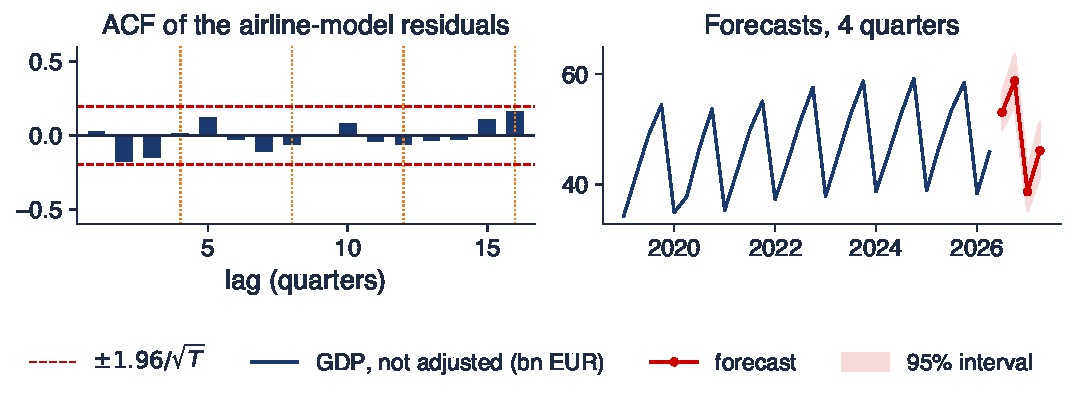
\includegraphics[width=0.96\textwidth,height=0.33\textheight,keepaspectratio]{ch4_sem_b1.pdf}
\end{center}
\vspace{-2mm}
\begin{itemize}
    \item $\hat\theta = -0.171$ (0.109): not significant; $\hat\Theta = -0.585$ (0.072); $\hat\sigma = 3.05\%$; $Q^*(8) = 9.30$, p = 0.157: no residual autocorrelation
    \item Forecasts from 2026Q3: 53.1, 58.7, 38.7, 46.1 bn EUR; first interval $[50.0, 56.4]$, fourth $[41.5, 51.2]$
    \item Implied year-on-year growth: $-$0.84\%, 0.52\%, 0.83\%, 0.53\%
    \item Interpretation: the seasonal forecast is an exponentially weighted average of past seasonal patterns, with weight $1 + \hat\Theta = 0.42$ on the newest year; $\Theta = -1$ would mean a fixed pattern, $\Theta = 0$ a pattern that changes freely: the pattern of GDP evolves slowly
\end{itemize}\quantlet{TSA\_ch4\_seminar}{\qlurl{TSA_ch4_seminar}}
\end{frame}

\begin{frame}{B2: industrial production and working days [Proposed]}
\itemsize{\footnotesize}
\begin{itemize}
\item \textbf{Question}: does the number of working days explain part of the monthly movements of Romanian industrial production?
\item \textbf{Inputs}: Eurostat, industrial production not adjusted, 2010--July 2026, $y_t = 100\ln Y_t$; dummies for April and May 2020; model: B1
\item \textbf{Tasks}
\begin{enumerate}
    \item Estimate the airline model with and without the number of working days as a regressor, and compare AICc and $Q^*(24)$.
    \item Add two alternatives with working days, $(2,1,0)(0,1,1)_{12}$ and $(1,1,1)(0,1,1)_{12}$, and choose a model.
    \item Report the working-day coefficient with its standard error, and forecast the next 12 months.
    \item Interpretation: why must the working-day effect be removed before two months are compared?
\end{enumerate}
\item \textbf{Report}: a table of AICc and p-values, one coefficient, the forecast chart and one sentence
\item Notebook: section B2
\end{itemize}
\end{frame}

\ifsolutions
\begin{frame}{B2: solution [Proposed]}
\itemsize{\scriptsize}
\begin{center}
\includegraphics[width=0.96\textwidth,height=0.30\textheight,keepaspectratio]{ch4_sem_b2.pdf}
\end{center}
\vspace{-2mm}
\begin{center}
\scriptsize
\begin{tabular}{lrr}
\toprule
Model & AICc & $Q^*(24)$, p \\
\midrule
$(0,1,1)(0,1,1)_{12}$ & 1023.8 & $<$\,0.001 \\
$(0,1,1)(0,1,1)_{12}$ + WD & \textbf{888.0} & 0.798 \\
$(2,1,0)(0,1,1)_{12}$ & 1012.0 & 0.003 \\
$(2,1,0)(0,1,1)_{12}$ + WD & 889.6 & 0.757 \\
$(1,1,1)(0,1,1)_{12}$ + WD & 890.1 & 0.742 \\
\bottomrule
\end{tabular}
\end{center}
\begin{itemize}
    \item Best: airline + working days (WD); one more working day raises production by 2.49\% (se 0.15); $\hat\theta = -0.481$, $\hat\Theta = -0.771$; without WD the residuals fail Ljung--Box and $\hat\Theta$ drifts to $-$0.998
    \item Interpretation: a month with two more working days has about 5.0\% more output for purely calendar reasons; comparing months without this correction mistakes the calendar for the business cycle
\end{itemize}
\end{frame}
\fi

\begin{frame}{B3: cross-validation for daily electricity load [Solved]}
\itemsize{\footnotesize}
\begin{itemize}
\item \textbf{Question}: does a regression with Fourier terms and holiday dummies forecast daily load better than SARIMA and the seasonal naive method?
\item \textbf{Inputs}: ENTSO-E, daily mean load in Romania (GW), 2022--2026; 13 origins every 28 days from 30 June 2025 to 1 June 2026, horizon 14 days
\item \textbf{Tasks}
\begin{enumerate}
    \item At each origin, fit the seasonal naive method (period 7), SARIMA$(1,0,1)(0,1,1)_7$ and a DHR (4 annual Fourier pairs, weekday and holiday dummies, ARMA(1,1) errors).
    \item Compute the MAE and the MASE of each method over all origins and horizons.
    \item Test DHR against SARIMA with the DM test on the window-average squared errors (one value per origin), with the HLN correction.
    \item Compare the MAE on public holidays with the MAE on ordinary days.
    \item Interpretation: why is the gain of the DHR largest on public holidays?
\end{enumerate}
\item \textbf{Report}: a table of MAE and MASE, one test, the chart and one sentence
\item Notebook: section B3
\end{itemize}
\end{frame}

\begin{frame}{B3: solution [Solved]}
\itemsize{\scriptsize}
\begin{center}
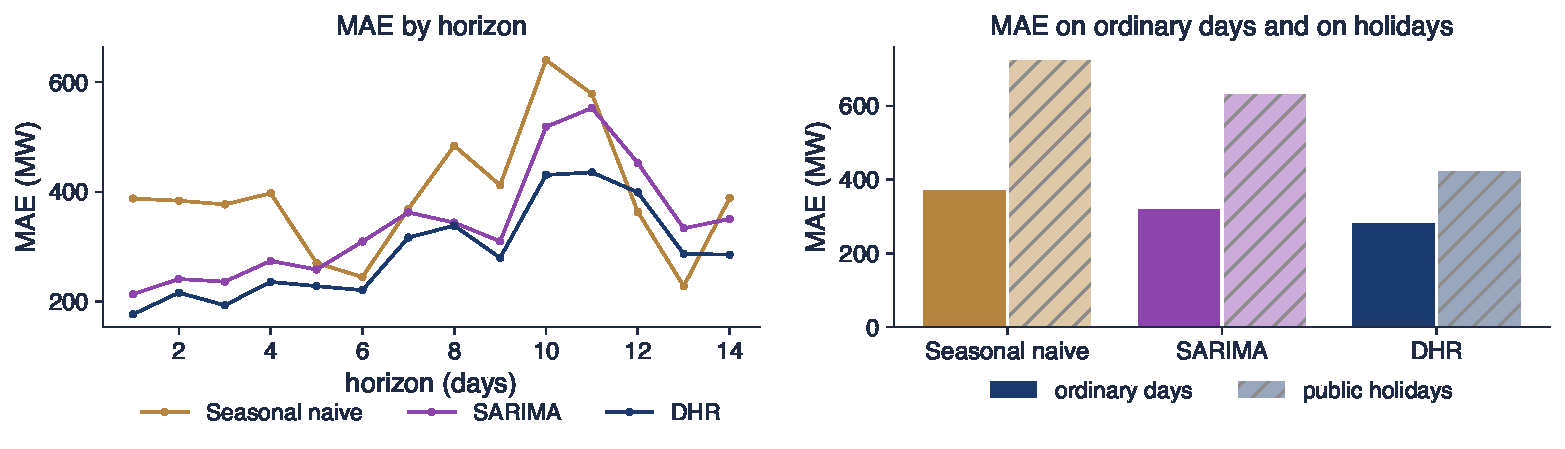
\includegraphics[width=0.96\textwidth,height=0.32\textheight,keepaspectratio]{ch4_sem_b3.pdf}
\end{center}
\vspace{-2mm}
\begin{center}
\scriptsize
\begin{tabular}{lrrrr}
\toprule
Method & MAE (MW) & MASE & holidays & other days \\
\midrule
Seasonal naive & 395 & 1.28 & 723 & 372 \\
SARIMA & 340 & 1.10 & 630 & 319 \\
DHR & \textbf{289} & \textbf{0.94} & 422 & 280 \\
\bottomrule
\end{tabular}
\end{center}
\begin{itemize}
    \item MASE scale: in-sample MAE of the weekly seasonal naive method, 309 MW; DM (HLN), DHR against SARIMA: $-$1.96, p = 0.073; against the seasonal naive method: $-$2.73, p = 0.018
    \item Interpretation: SARIMA and the seasonal naive method only know ``one week ago''; a holiday that falls on a weekday looks to them like a normal working day, while the DHR has dummies that remove 0.37 GW on a public holiday and 0.56 GW on the Easter days
\end{itemize}\quantlet{TSA\_ch4\_seminar}{\qlurl{TSA_ch4_seminar}}
\end{frame}

\begin{frame}{B4: seasonality in monthly inflation [Proposed]}
\itemsize{\footnotesize}
\begin{itemize}
\item \textbf{Question}: is the seasonal pattern of Romanian monthly inflation strong enough to improve one-month forecasts?
\item \textbf{Inputs}: HICP, Romania, 2010--2026; $\pi_t = 100\,\Delta\ln P_t$ (\% per month); model: B3
\item \textbf{Tasks}
\begin{enumerate}
    \item Regress $\pi_t$ (2010--2019) on 12 month dummies and test equal month means with an $F$-test.
    \item Estimate the airline model for $100\ln P_t$ and report $\hat\theta$ and $\hat\Theta$.
    \item From monthly origins since January 2016, forecast next month's $\pi$ with SARIMA, the seasonal naive method and the mean of the last 12 months; compare the MAE.
    \item Test SARIMA against both benchmarks with the DM test (squared errors).
    \item Interpretation: is the seasonal pattern strong enough to improve one-month forecasts?
\end{enumerate}
\item \textbf{Report}: an $F$-test, two estimates, three MAE values, two DM tests and one sentence
\item Notebook: section B4
\end{itemize}
\end{frame}

\ifsolutions
\begin{frame}{B4: solution [Proposed]}
\itemsize{\scriptsize}
\begin{center}
\includegraphics[width=0.96\textwidth,height=0.30\textheight,keepaspectratio]{ch4_sem_b4.pdf}
\end{center}
\vspace{-2mm}
\begin{itemize}
    \item $F = 2.71$, p = 0.004: the month means differ; January 0.45\%, June $-$0.37\% (fresh food), August $-$0.10\%, October 0.49\%
    \item Airline: $\hat\theta = 0.356$ (0.060), $\hat\Theta = -0.782$ (0.063); 127 forecasts, February 2016--August 2026: MAE SARIMA 0.312, seasonal naive 0.427, mean of 12 months 0.313
    \item DM (HLN): SARIMA against the seasonal naive method $-$3.27 (p = 0.001); against the 12-month mean 0.08 (p = 0.935)
    \item Interpretation: the seasonal pattern is real but small next to the monthly noise; SARIMA beats copying last year's month, yet it does not beat the simple 12-month mean
\end{itemize}
\end{frame}
\fi


%=============================================================================
\section{Part C: open questions and AI critique}
%=============================================================================

\begin{frame}{C1: tourism after the pandemic [Proposed]}
\itemsize{\footnotesize}
\begin{itemize}
\item \textbf{Question}: which training sample gives better forecasts of tourism nights for 2023--2025: data up to 2019, or data up to 2022?
\item \textbf{Inputs}: Eurostat, nights in tourist accommodation, Romania, monthly, 2005--2025; model: B1
\item \textbf{Tasks}
\begin{enumerate}
    \item Fit the airline model to $\ln y_t$ up to December 2019 and forecast 2023--2025.
    \item Repeat with data up to December 2022.
    \item Compare both with the seasonal naive forecast that repeats 2022, using the MAPE (mean absolute percentage error).
    \item Propose a better treatment of 2020--2021 (intervention dummies, a shorter sample, TBATS or Prophet) and sketch it as a team project.
\end{enumerate}
\item \textbf{Report}: three MAPE values, the chart and a project plan
\item Notebook: section C1
\end{itemize}
\end{frame}

\ifsolutions
\begin{frame}{C1: reference analysis [Proposed]}
\itemsize{\scriptsize}
\begin{center}
\includegraphics[width=0.96\textwidth,height=0.36\textheight,keepaspectratio]{ch4_sem_c1.pdf}
\end{center}
\vspace{-2mm}
\begin{itemize}
    \item MAPE 2023--2025: airline trained to 2019 20.0\%; trained to 2022 37.7\%; seasonal naive (2022 repeated) 11.6\%; nights: 29.9 million in 2019, 29.7 million in 2025
    \item Interpretation: the collapse of 2020 enters the differenced data as huge shocks, and the model trained to 2022 extrapolates the rebound; the old model ignores the break; the simplest forecast wins. A project: intervention analysis with dummies for 2020--2021, compared by rolling origins
\end{itemize}
\end{frame}
\fi

\begin{frame}{C2: audit an AI answer [Proposed]}
\itemsize{\scriptsize}
\begin{itemize}
    \item A student asked an AI assistant about seasonal models. The answer:
    \item \aiprompt{(a) SARIMA(0,1,1)(0,1,1)4 has four MA parameters, at lags 1, 4 and 5 plus the noise variance.}
    \item \aiprompt{(b) If the ACF of the differenced monthly series has one spike at lag 12 and the PACF decays at 12, 24, 36, use a seasonal AR(1).}
    \item \aiprompt{(c) Unadjusted Romanian GDP fell by about 34\% in the first quarter of 2026 compared with the fourth quarter of 2025: a deep recession.}
    \item \aiprompt{(d) DM = $-$2.3 with d = L(e1) - L(e2) shows that forecast 2 is significantly more accurate.}
    \item \aiprompt{(e) TBATS with periods 7 and 365.25 captures the Easter dip of electricity load.}
    \item \aiprompt{(f) The equal-weight average of two unbiased forecasts never has a larger MSE than the average of their two MSEs.}
    \item Tasks
    \begin{itemize}
        \item 1. For each statement, say whether it is correct; if not, give the correct statement and, where possible, the correct number from the notebook (section C2).
        \item 2. Report: a list of six verdicts with one line of justification each.
    \end{itemize}
\end{itemize}
\end{frame}

\ifsolutions
\begin{frame}{C2: solution [Proposed]}
\itemsize{\scriptsize}
\begin{itemize}
    \item (a) Wrong: two MA parameters, $\theta$ and $\Theta$; the lag-5 coefficient is the product $\theta\Theta$ (A2, A3)
    \item (b) Wrong: an ACF that cuts off at lag 12 with a decaying seasonal PACF is a seasonal MA(1) (A4)
    \item (c) Wrong: the fall is seasonal (Q1 is always the lowest quarter): unadjusted $-$34.3\%, adjusted (SCA) $-$0.06\% in 2026Q1
    \item (d) Wrong: $\bar d < 0$ favours forecast 1; significance also needs $|\mathrm{HLN}|$ above the $t(n - 1)$ critical value (A5)
    \item (e) Wrong: Orthodox Easter moves between April and May; a fixed period cannot follow it; it needs a holiday regressor, as in the DHR of B3
    \item (f) Correct: $\mathrm{MSE}(0.5) = (\sigma_1^2 + \sigma_2^2 + 2\rho\sigma_1\sigma_2)/4 \le (\sigma_1^2 + \sigma_2^2)/2$, because $2\rho\sigma_1\sigma_2 \le \sigma_1^2 + \sigma_2^2$ (A6)
\end{itemize}\quantlet{TSA\_ch4\_seminar}{\qlurl{TSA_ch4_seminar}}
\end{frame}
\fi


%=============================================================================
\section{Wrap-up}
%=============================================================================

\begin{frame}{Key takeaways}
\itemsize{\small}
\begin{itemize}
    \item $\Delta_s$ removes a stable seasonal pattern; $\Delta\Delta_s$ also removes the trend; the seasonal naive forecast is the benchmark
    \item SARIMA multiplies a regular and a seasonal polynomial: the airline model has two parameters and ACF spikes at $1$, $s - 1$, $s$, $s + 1$
    \item Calendar effects (working days, Easter, public holidays) are known in advance: put them in as regressors
    \item Compare forecasts out of sample, with rolling origins, MASE and the DM test; a visible gain is not always a significant one
    \item Combining forecasts is cheap insurance: it is rarely the worst and often near the best
\end{itemize}
\end{frame}

\begin{frame}{After the seminar}
\itemsize{\small}
\begin{itemize}
    \item Lecture 4 derives today's formulas and adds seasonal unit roots, seasonal adjustment (X-13ARIMA-SEATS), multiple seasonality, TBATS and Prophet
    \item Try the [Proposed] tasks in the notebook; TBATS and Prophet are optional installs there
    \item C1 can grow into a team project: forecasting tourism or electricity load in Romania with a rolling-origin comparison of several models
    \item Reading: \refHP, Ch.~4--5; \refFPPsar; \refFPPcv; \refDM
    \item \textbf{The seminar is for practice and is not graded; the solutions of [Proposed] tasks are discussed in class}
\end{itemize}
\end{frame}


%=============================================================================
\section{References}
%=============================================================================

\begin{frame}{References}
\itemsize{\tiny}
\begin{itemize}
    \item Bates, J. M., \& Granger, C. W. J. (1969). The combination of forecasts. \textit{Journal of the Operational Research Society}, 20(4), 451--468. \href{https://doi.org/10.1057/jors.1969.103}{doi:10.1057/jors.1969.103}
    \item Box, G. E. P., Jenkins, G. M., \& Reinsel, G. C. (2008). \textit{Time Series Analysis: Forecasting and Control} (4th ed.). Wiley. \href{https://doi.org/10.1002/9781118619193}{doi:10.1002/9781118619193}
    \item Diebold, F. X., \& Mariano, R. S. (1995). Comparing predictive accuracy. \textit{Journal of Business \& Economic Statistics}, 13(3), 253--263. \href{https://doi.org/10.1080/07350015.1995.10524599}{doi:10.1080/07350015.1995.10524599}
    \item Harvey, D., Leybourne, S., \& Newbold, P. (1997). Testing the equality of prediction mean squared errors. \textit{International Journal of Forecasting}, 13(2), 281--291. \href{https://doi.org/10.1016/S0169-2070(96)00719-4}{doi:10.1016/S0169-2070(96)00719-4}
    \item Huang, C., \& Petukhina, A. (2022). \textit{Applied Time Series Analysis and Forecasting with Python}. Springer. \href{https://doi.org/10.1007/978-3-031-13584-2}{doi:10.1007/978-3-031-13584-2}
    \item Hyndman, R. J., \& Athanasopoulos, G. (2021). \textit{Forecasting: Principles and Practice} (3rd ed.). OTexts. \href{https://otexts.com/fpp3/}{otexts.com/fpp3}
    \item Hyndman, R. J., \& Koehler, A. B. (2006). Another look at measures of forecast accuracy. \textit{International Journal of Forecasting}, 22(4), 679--688. \href{https://doi.org/10.1016/j.ijforecast.2006.03.001}{doi:10.1016/j.ijforecast.2006.03.001}
    \item Ljung, G. M., \& Box, G. E. P. (1978). On a measure of lack of fit in time series models. \textit{Biometrika}, 65(2), 297--303. \href{https://doi.org/10.1093/biomet/65.2.297}{doi:10.1093/biomet/65.2.297}
    \item Tashman, L. J. (2000). Out-of-sample tests of forecasting accuracy: an analysis and review. \textit{International Journal of Forecasting}, 16(4), 437--450. \href{https://doi.org/10.1016/S0169-2070(00)00065-0}{doi:10.1016/S0169-2070(00)00065-0}
\end{itemize}
\end{frame}

\end{document}
